\chapter{Synchronizacja czasu}

Synchronizacja czasu jest jednym z podstawowych problemów systemów opartych o wiele urządzeń posiadających własne zegary. Wiedza o dokładnym czasie zachodzących w sieci zdarzeń jest niezbędna do szybkiego przesyłu danych, koordynacji procesów czy aktualizacji systemu plików. W przypadku niniejszej pracy dokładne określenie czasu zachodzących zdarzeń jest kluczowe do wiarygodnego określenia odległości pomiędzy węzłami na podstawie interwału czasowego pomiędzy nadaniem a odbiorem sygnału dźwiękowego.

\section{Synchronizacja programowa}

Pierwszym podejściem do rozwiązania problemu synchronizacji zegarów było zastosowanie synchronizacji programowej~\cite{6066334}, w której urządzenie-host utrzymuje wysokiej rozdzielczości licznik czasowy i wysyła sygnały o jego wartości pozostałym węzłom w sieci. Na podstawie tych informacji każdy z węzłów oblicza różnicę w zegarach i wprowadza odpowiednie przesunięcie własnego licznika.

\subsection{Algorytm synchronizacji NTP}

Jednym z najbardziej rozpowszechnionych protokołów synchronizacji programowej jest \textit{Network Time Protocol} opisany w pracy~\cite{103043}. Zachowując oznaczenia w niej zastosowane opiszmy w skrócie zasadę działania tego protokołu.

Na rysunku~\ref{fig:ntp} przestawiono schemat działania protokołu NTP. Urządzenia \textit{A} i \textit{B} wymieniają wiadomości zawierające sygnatury czasowe. Niech $T_{i},\ T_{i-1},\ T_{i-2},\ T_{i-3}$ będą czterema ostatnimi wiadomościami oraz niech $a = T_{i-2} - T_{i-3}$ oraz $b = T_{i-1} - T_i$. Wtedy całkowity czas transmisji $\delta_i$ i przesunięcie zegara $\theta_i$ urządzenia \textit{B} względem urządzenia \textit{A} to

\[\delta_i = a - b\quad \text{oraz}\quad \theta_i = \frac{a+b}{2}\]

Dodatkowym wnioskiem przedstawionym w powyższej pracy jest własność prawdziwego przesunięcia względem aktualnie obliczonego:

\[\theta_i - \frac{\delta_i}{2} \leq \theta \leq \theta_i + \frac{\delta_i}{2}\]

Jak łatwo zauważyć im krótszy jest czas propagacji tym lepsze przybliżenie dostajemy.

\begin{figure}[h]
    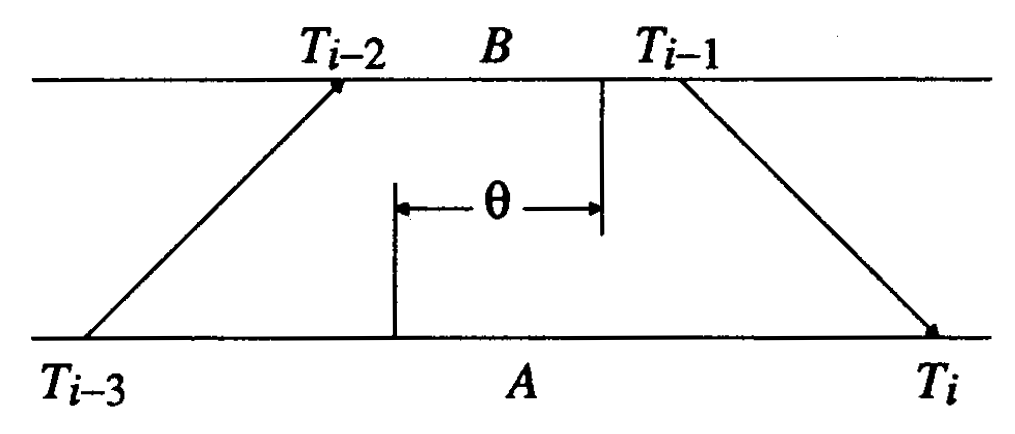
\includegraphics[width=\textwidth]{pics/ntp.png}
\caption{Pomiar opóźnienia transmisji i przesunięcia zegara}
\label{fig:ntp}
\end{figure}

Na postawie tych informacji podjęto próbę synchronizacji programowej zegarów węzłów w systemie multilateracyjnym. Przy użyciu czterech węzłów przeprowadzono eksperymenty mające na celu próbę ustalenia przesunięć zegarów każdego z urządzeń względem centralnego serwera. Opisany wyżej schemat wymiany czterech wiadomości powtarzano $n$ razy wspólnie dla wszystkich węzłów zapisując obliczone przesunięcia oraz czasy propagacji.

W celu poprawy czytelności wyniki przesunięć zostały znormalizowane poprzez przesunięcie o wartość średnią dla każdego z węzłów.

\begin{figure}[h]
\centering
    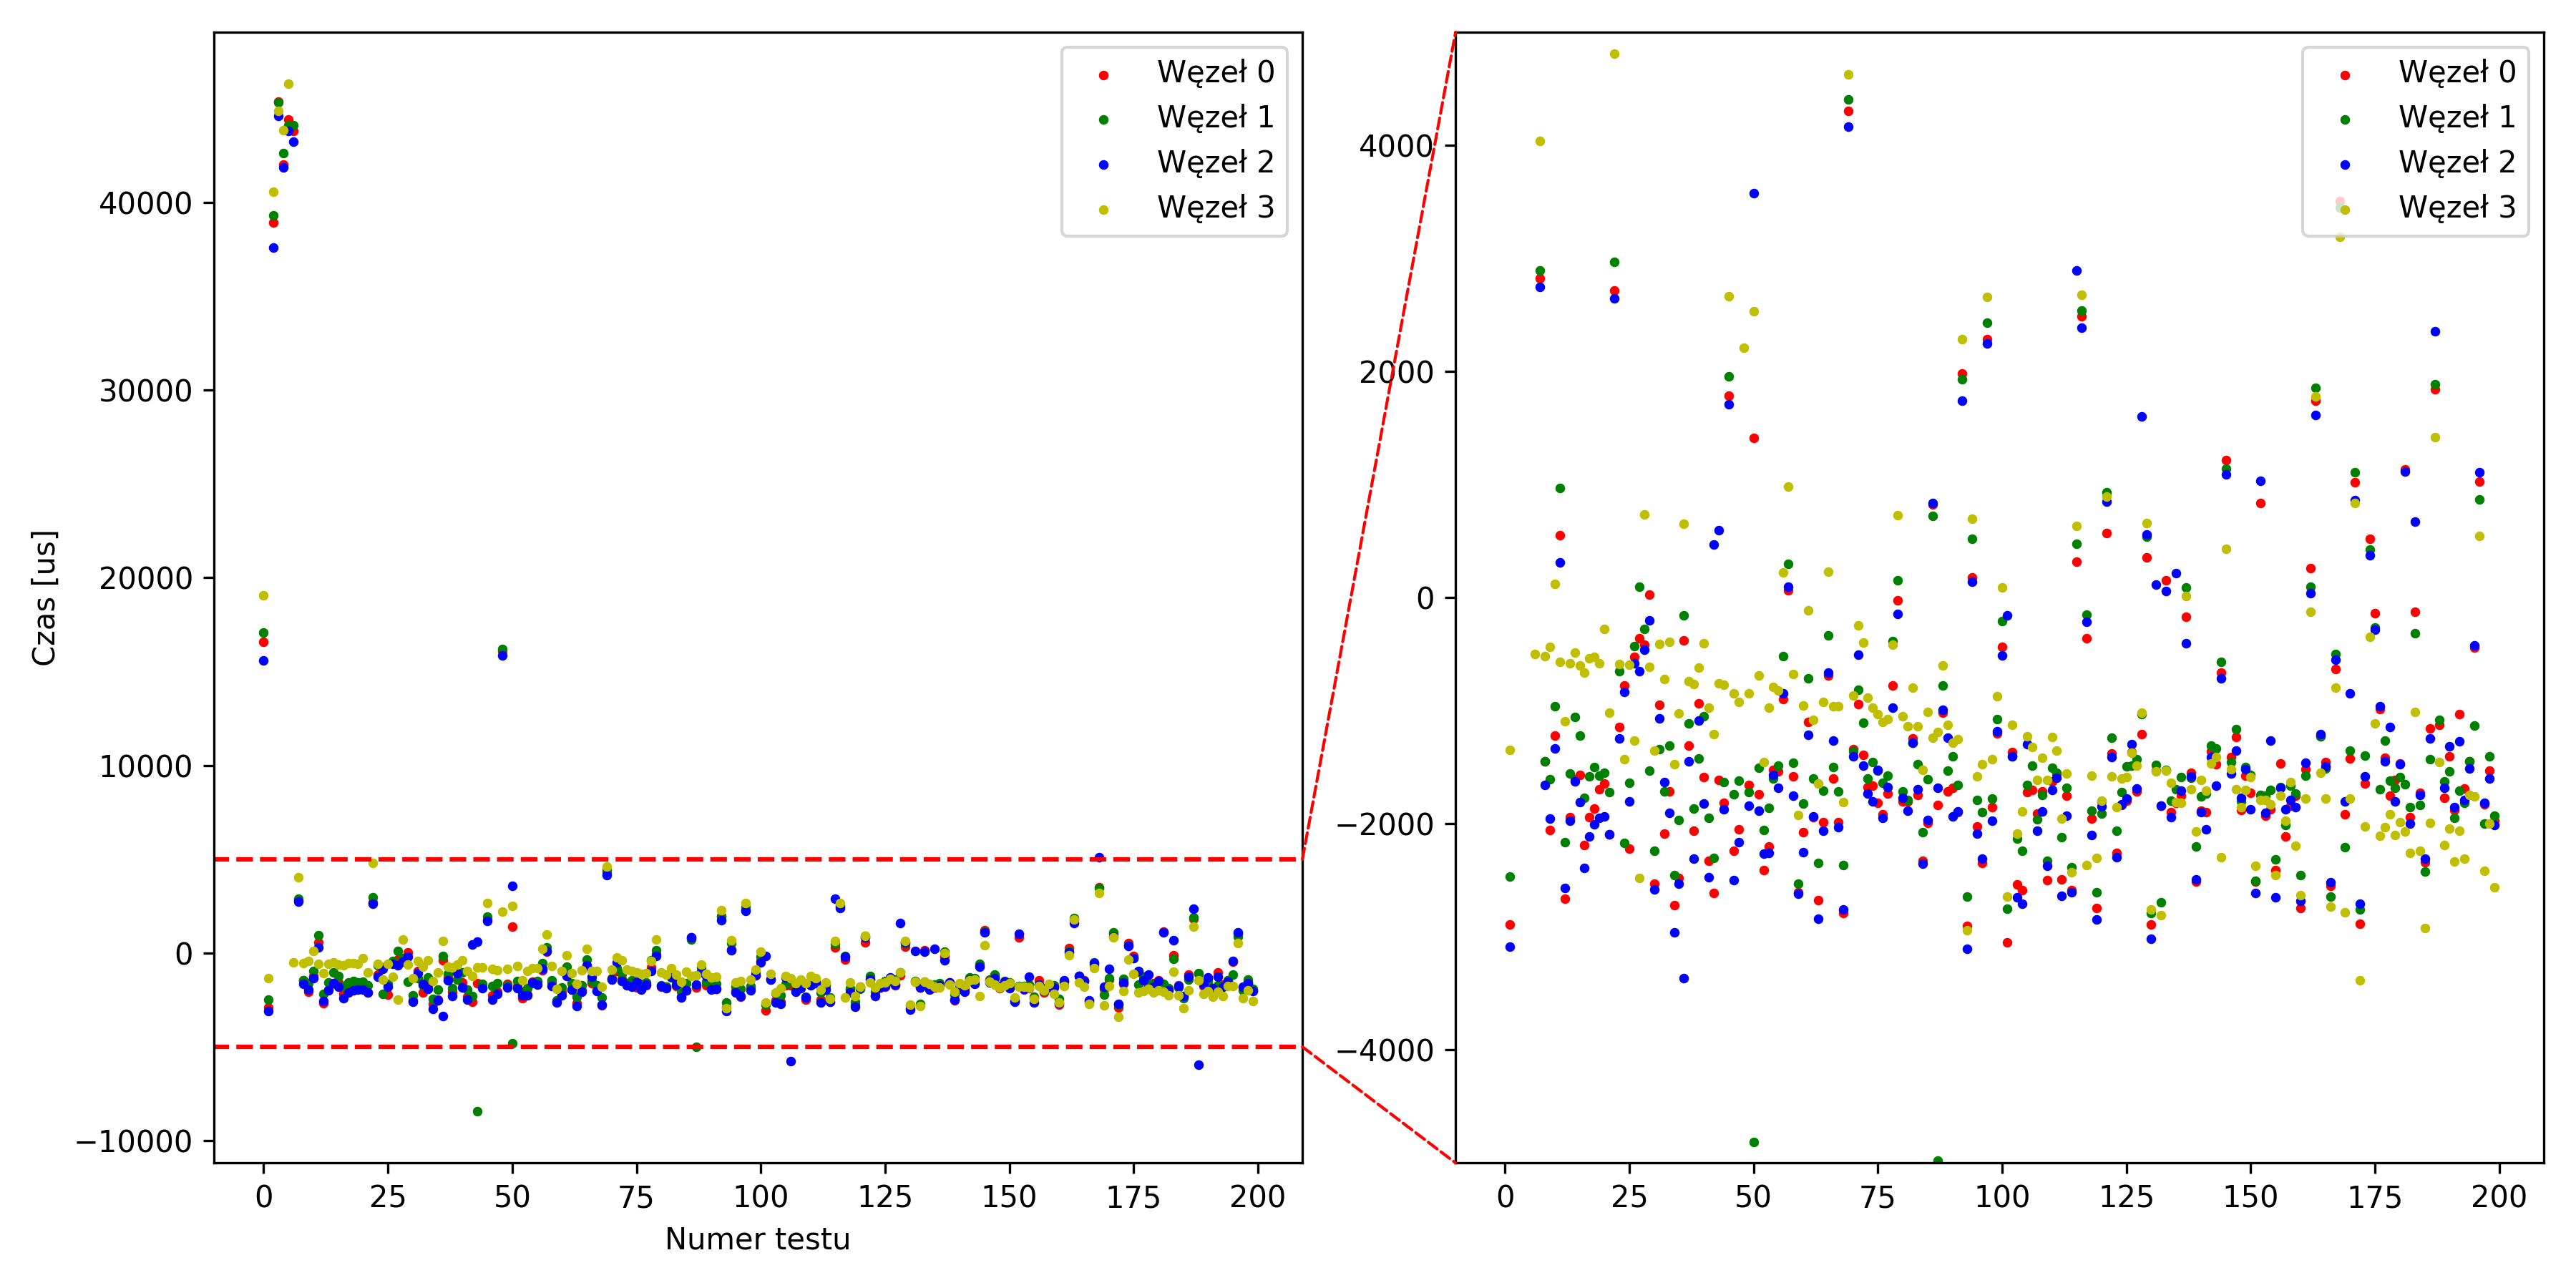
\includegraphics[width=.49\textwidth]{pics/ntp_sync/offsets.png}
    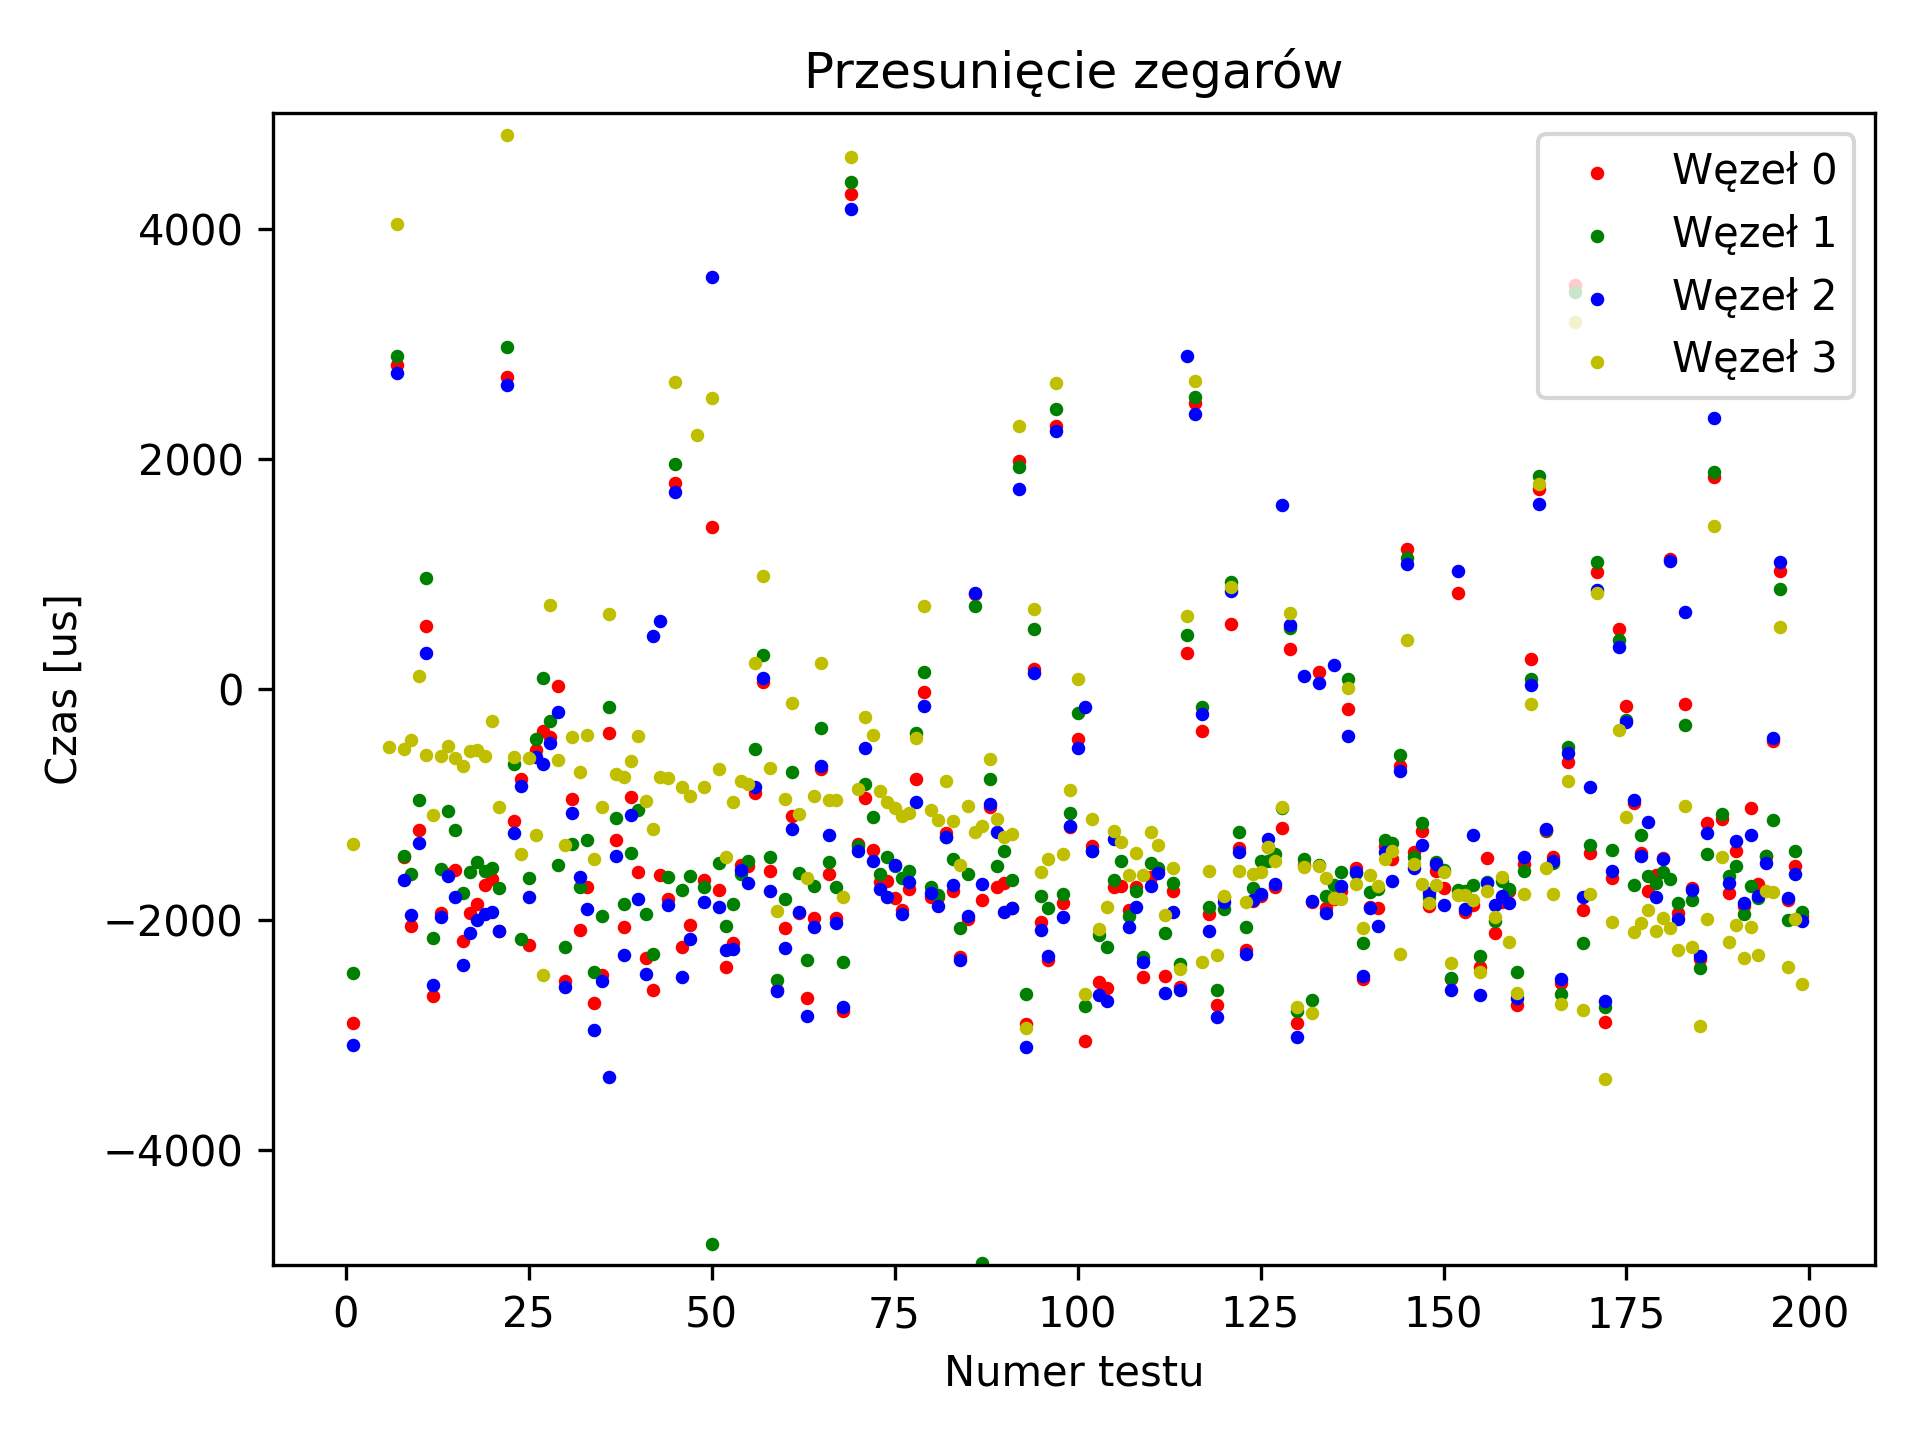
\includegraphics[width=.49\textwidth]{pics/ntp_sync/offsets_close.png}
\caption{Wyniki pomiarów przesunięć zegarów}
\label{pic:offsets_ntp}
\end{figure}

\begin{figure}[h]
\centering
    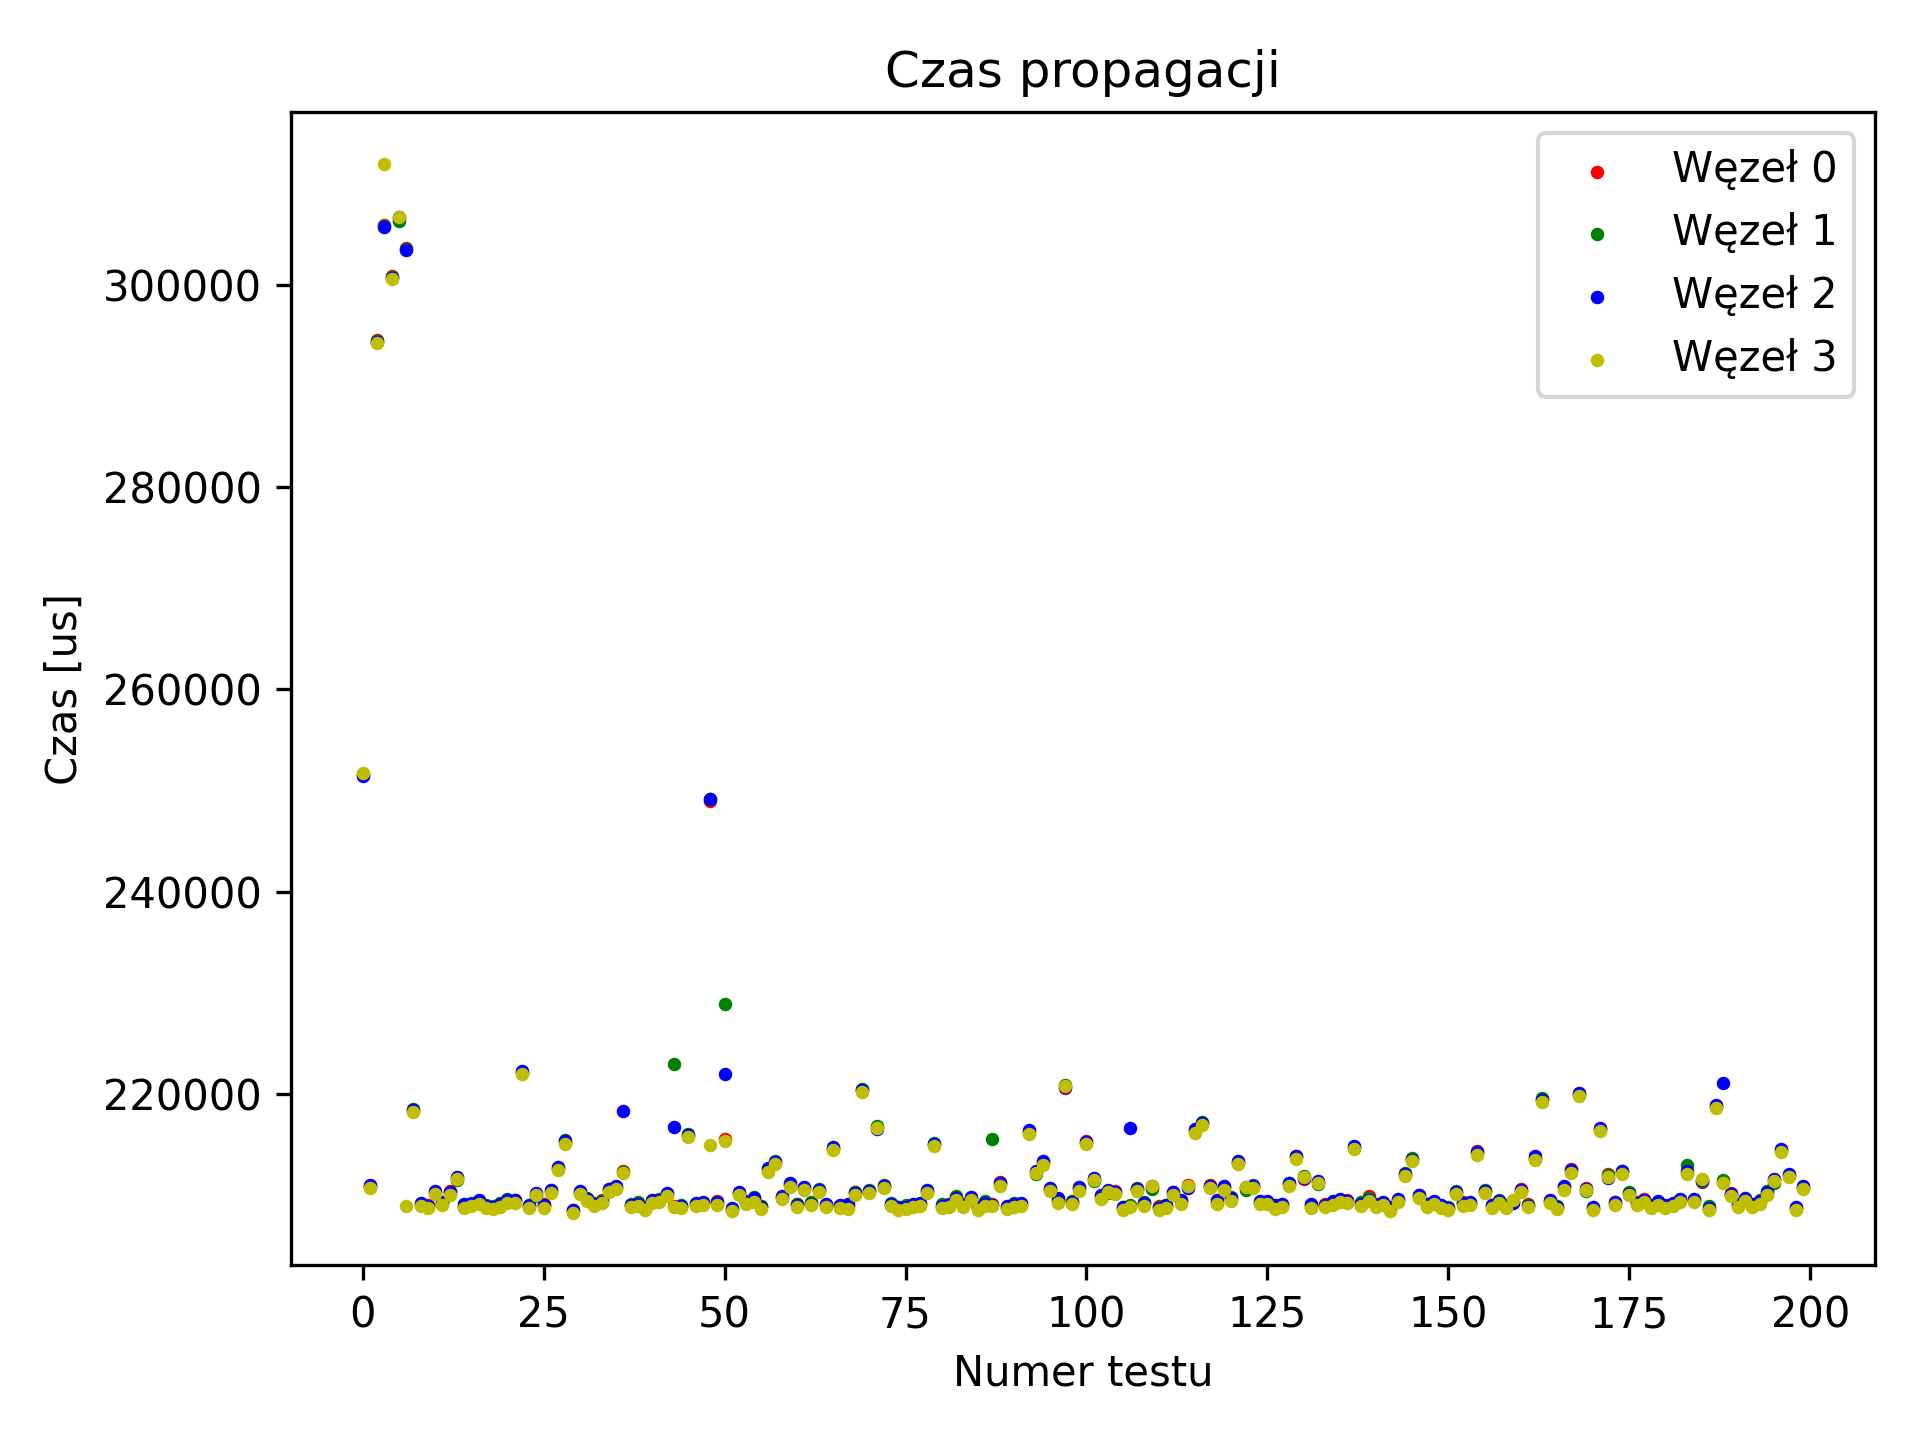
\includegraphics[width=.49\textwidth]{pics/ntp_sync/prop_times.png}
    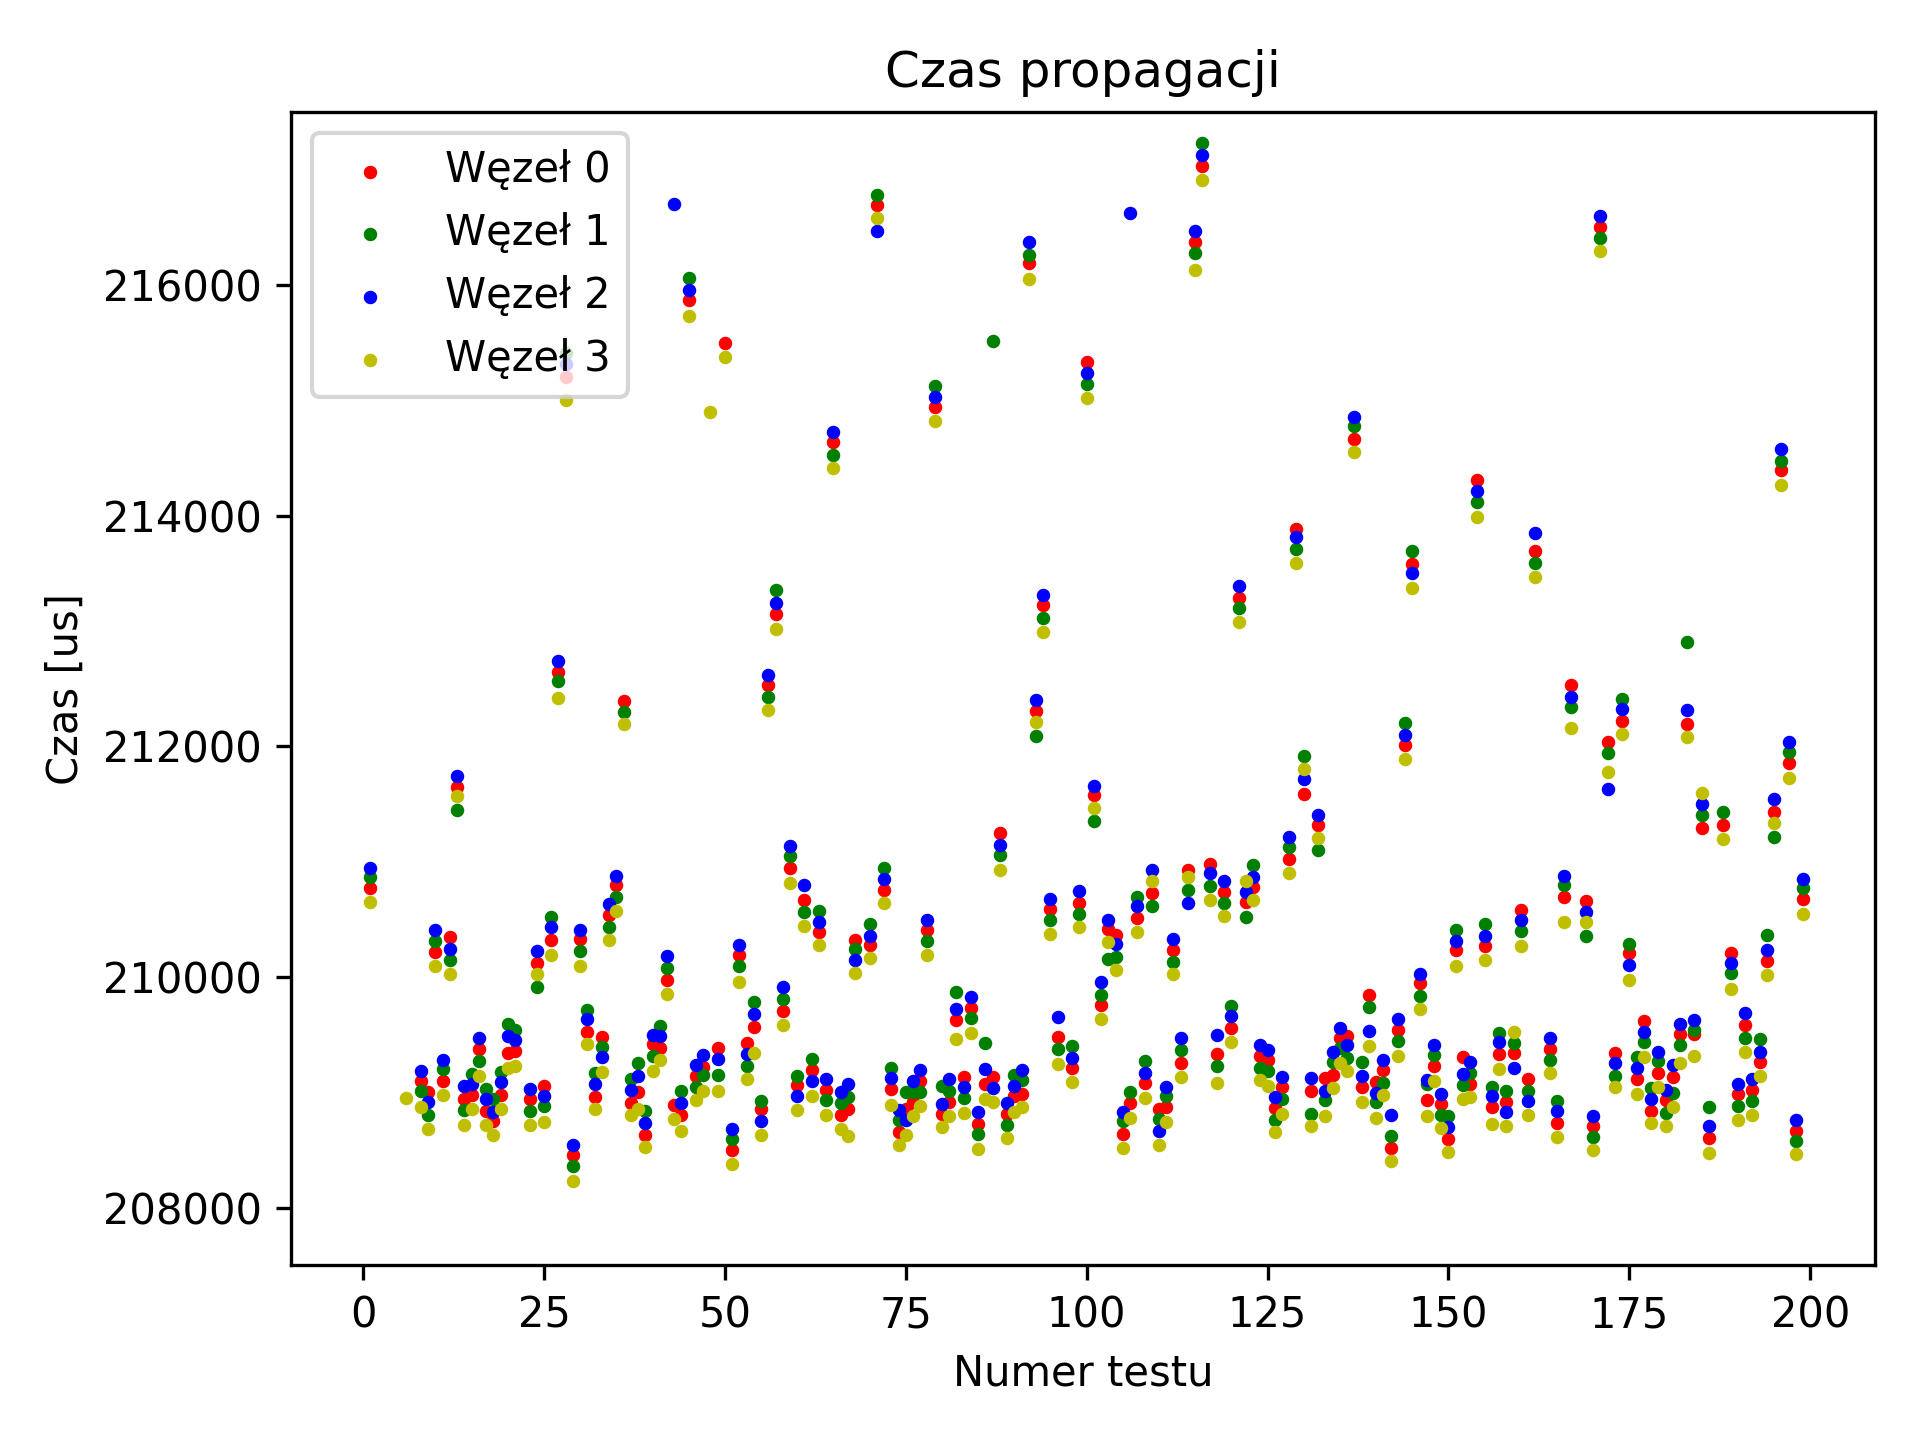
\includegraphics[width=.49\textwidth]{pics/ntp_sync/prop_times_close.png}
\caption{Wyniki pomiarów czasów propagacji}
\label{pic:prop_times}
\end{figure}

\begin{figure}[h]
\centering
    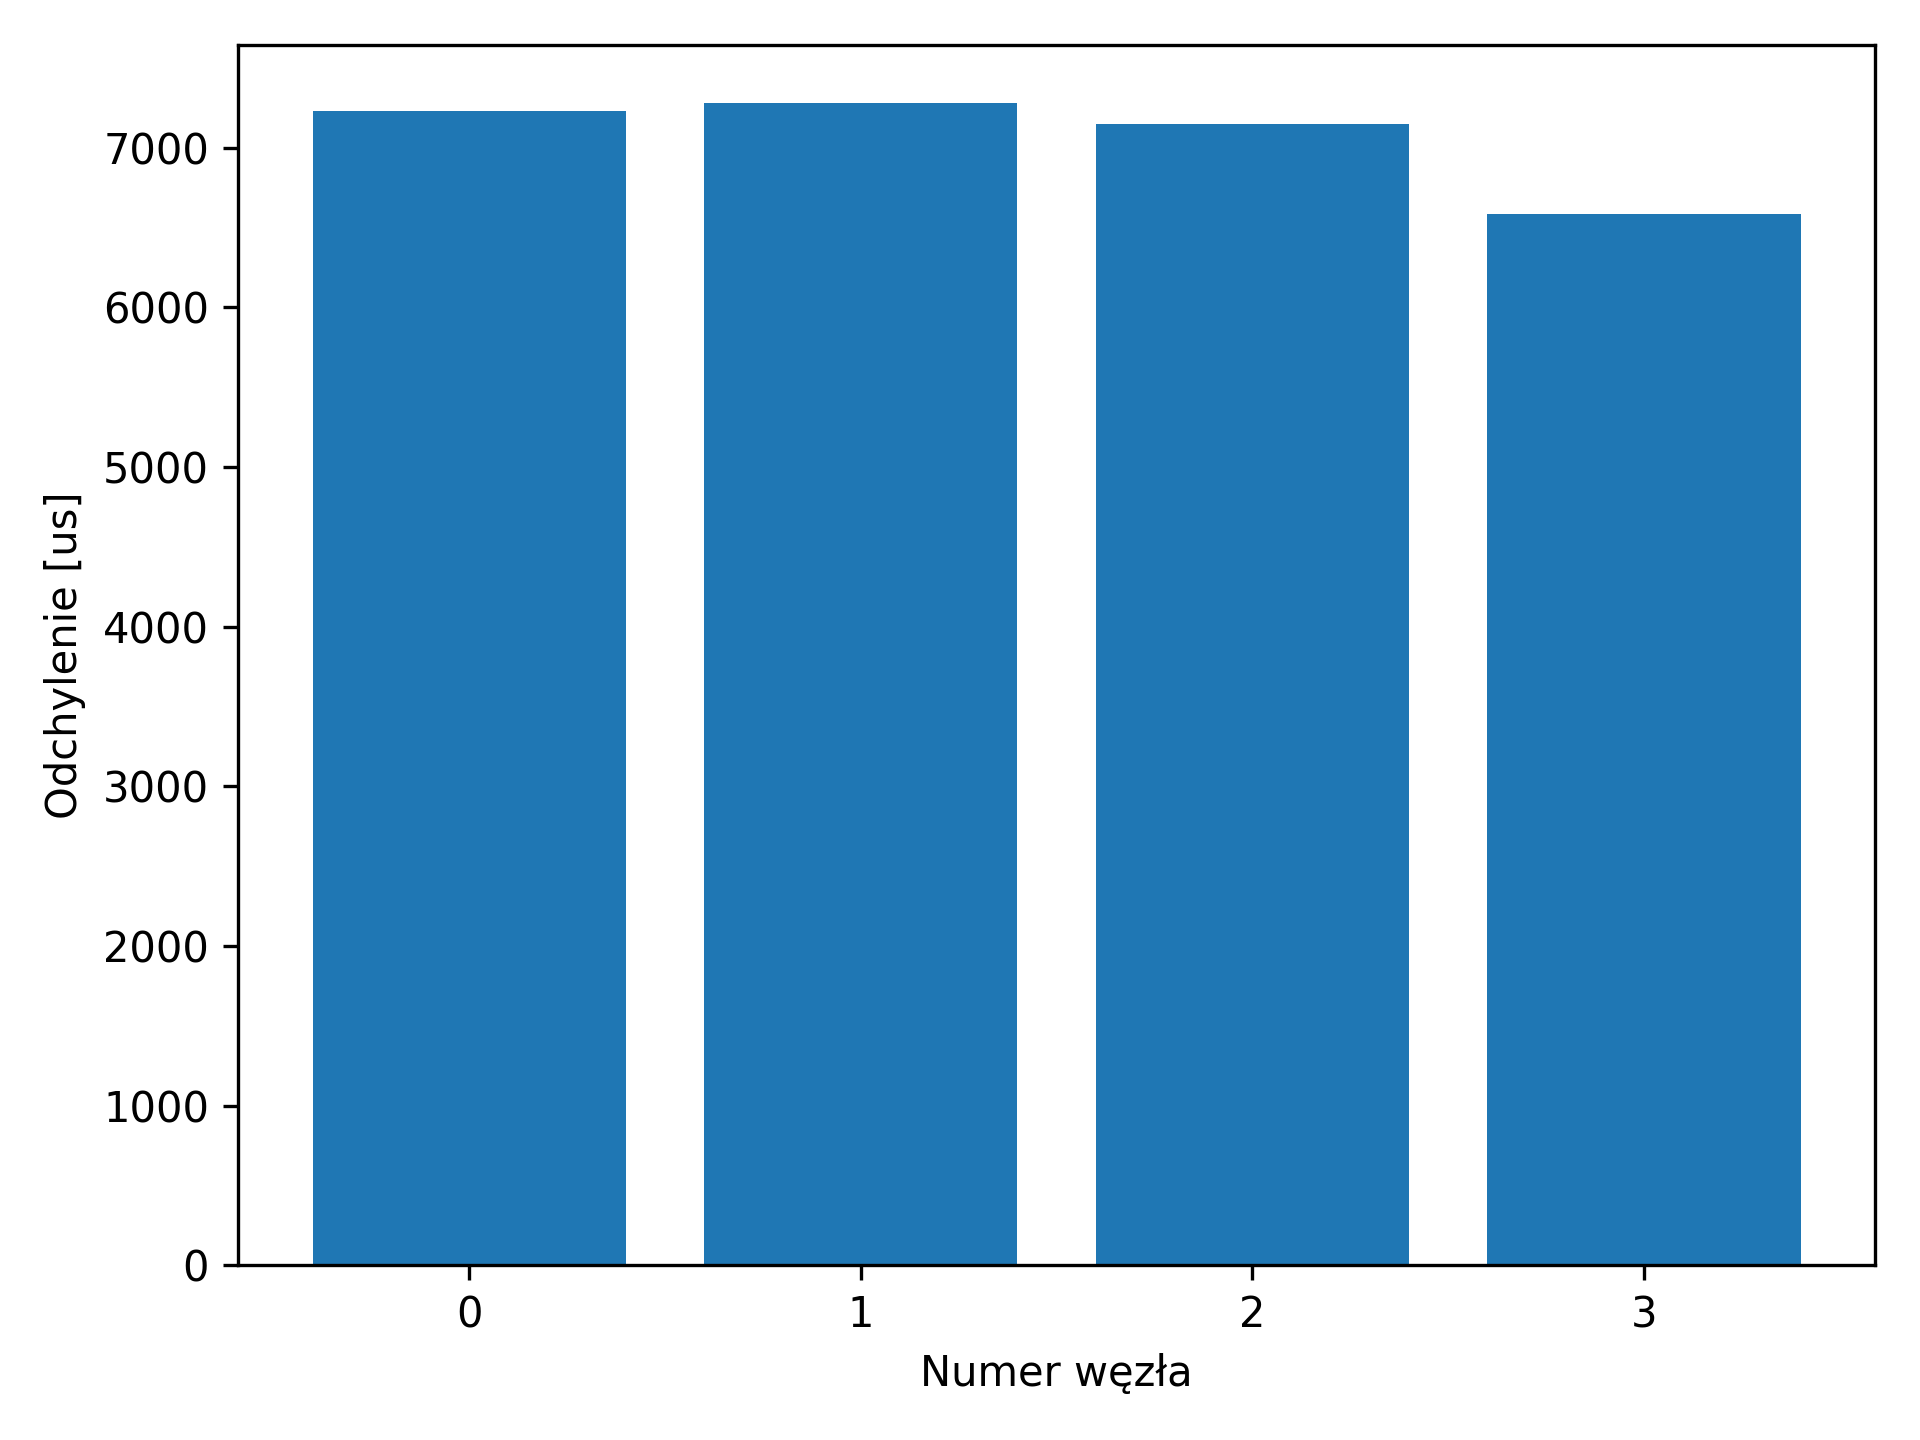
\includegraphics[width=.49\textwidth]{pics/ntp_sync/stddev_offsets.png}
    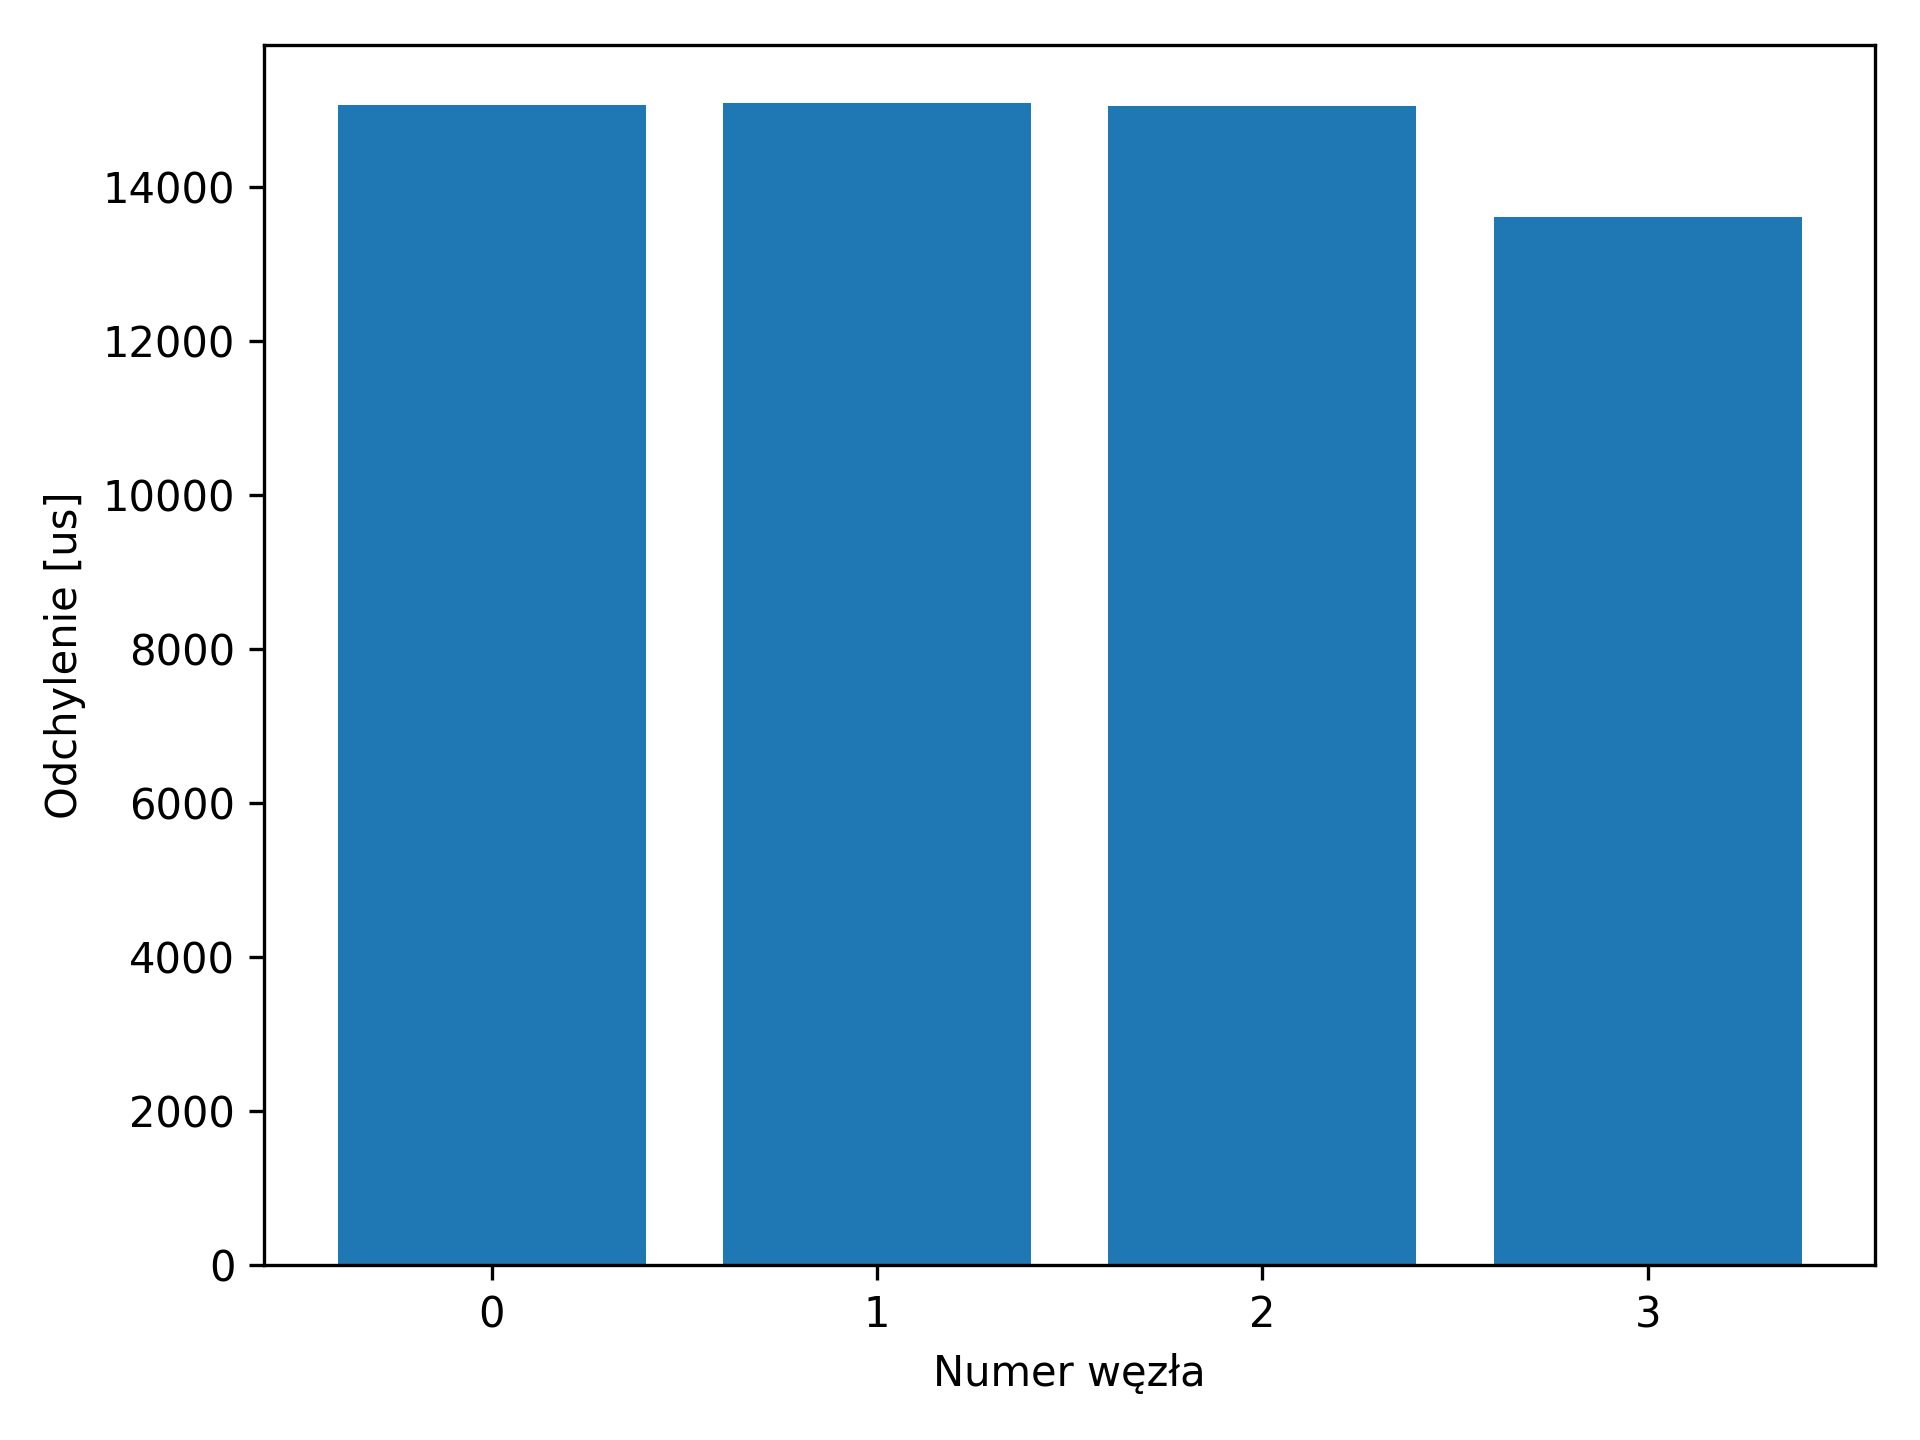
\includegraphics[width=.49\textwidth]{pics/ntp_sync/stddev_prop.png}
\caption{Odchylenia standardowe pomiarów}
\label{pic:stddev_ntp}
\end{figure}

Na podstawie otrzymanych wykresów łatwo zauważyć, że czas propagacji wiadomości w systemie jest nieprzewidywalny i zmienia sie znacząco z pomiaru na pomiar. Interesującą nas statystyką są jednak zaobserwowane przesunięcia zegarów, bez których nie jesteśmy w stanie poprawnie ocenić odległości od źródła dźwięku. Tutaj wartości wyglądają na bardziej skoncentrowane, jednak nie widać wyraźnych tendencji koncentracji wokół wartości średnich dla żadnego z węzłów. Ponadto zaobserwowane odchylenia standardowe $\sigma_i,\ i \in \{0,1,2,3\}$ wielkości $\approx 7000 \mu s$ są nieakceptowalne, ponieważ w takim czasie dźwięk w powietrzu pokonuje $\frac{7000}{1000000}s \cdot 343\frac{m}{s} = 2.401m$. Możliwe jest, że wielokrotne powtarzanie pomiarów da zadowalającą wartość średnią, pozwalającą na centymetrową precyzję obliczanych odległości. W porównaniu z pozostałymi sposobami brane będą pod uwagę wartości uśrednione.

\subsection{Bezpośredni pomiar przesunięć zegarów}

Biorąc pod uwagę zauważoną nieprzewidywalność i rozrzut czasów propagacji (spowodowanych najprawdopodobniej użyciem protokołu MQTT do przesyłu wiadomości pomiędzy urządzeniami) następnym pomysłem schematu synchronizacji jest bezpośrednie badanie względnego przesunięcia zegarów. Węzeł wysyła $n$ wiadomości zawierających aktualną wartość zegara, która po odebraniu przez serwer jest porównywana z zegarem w nim dostępnym.

\begin{figure}[h]
\centering
    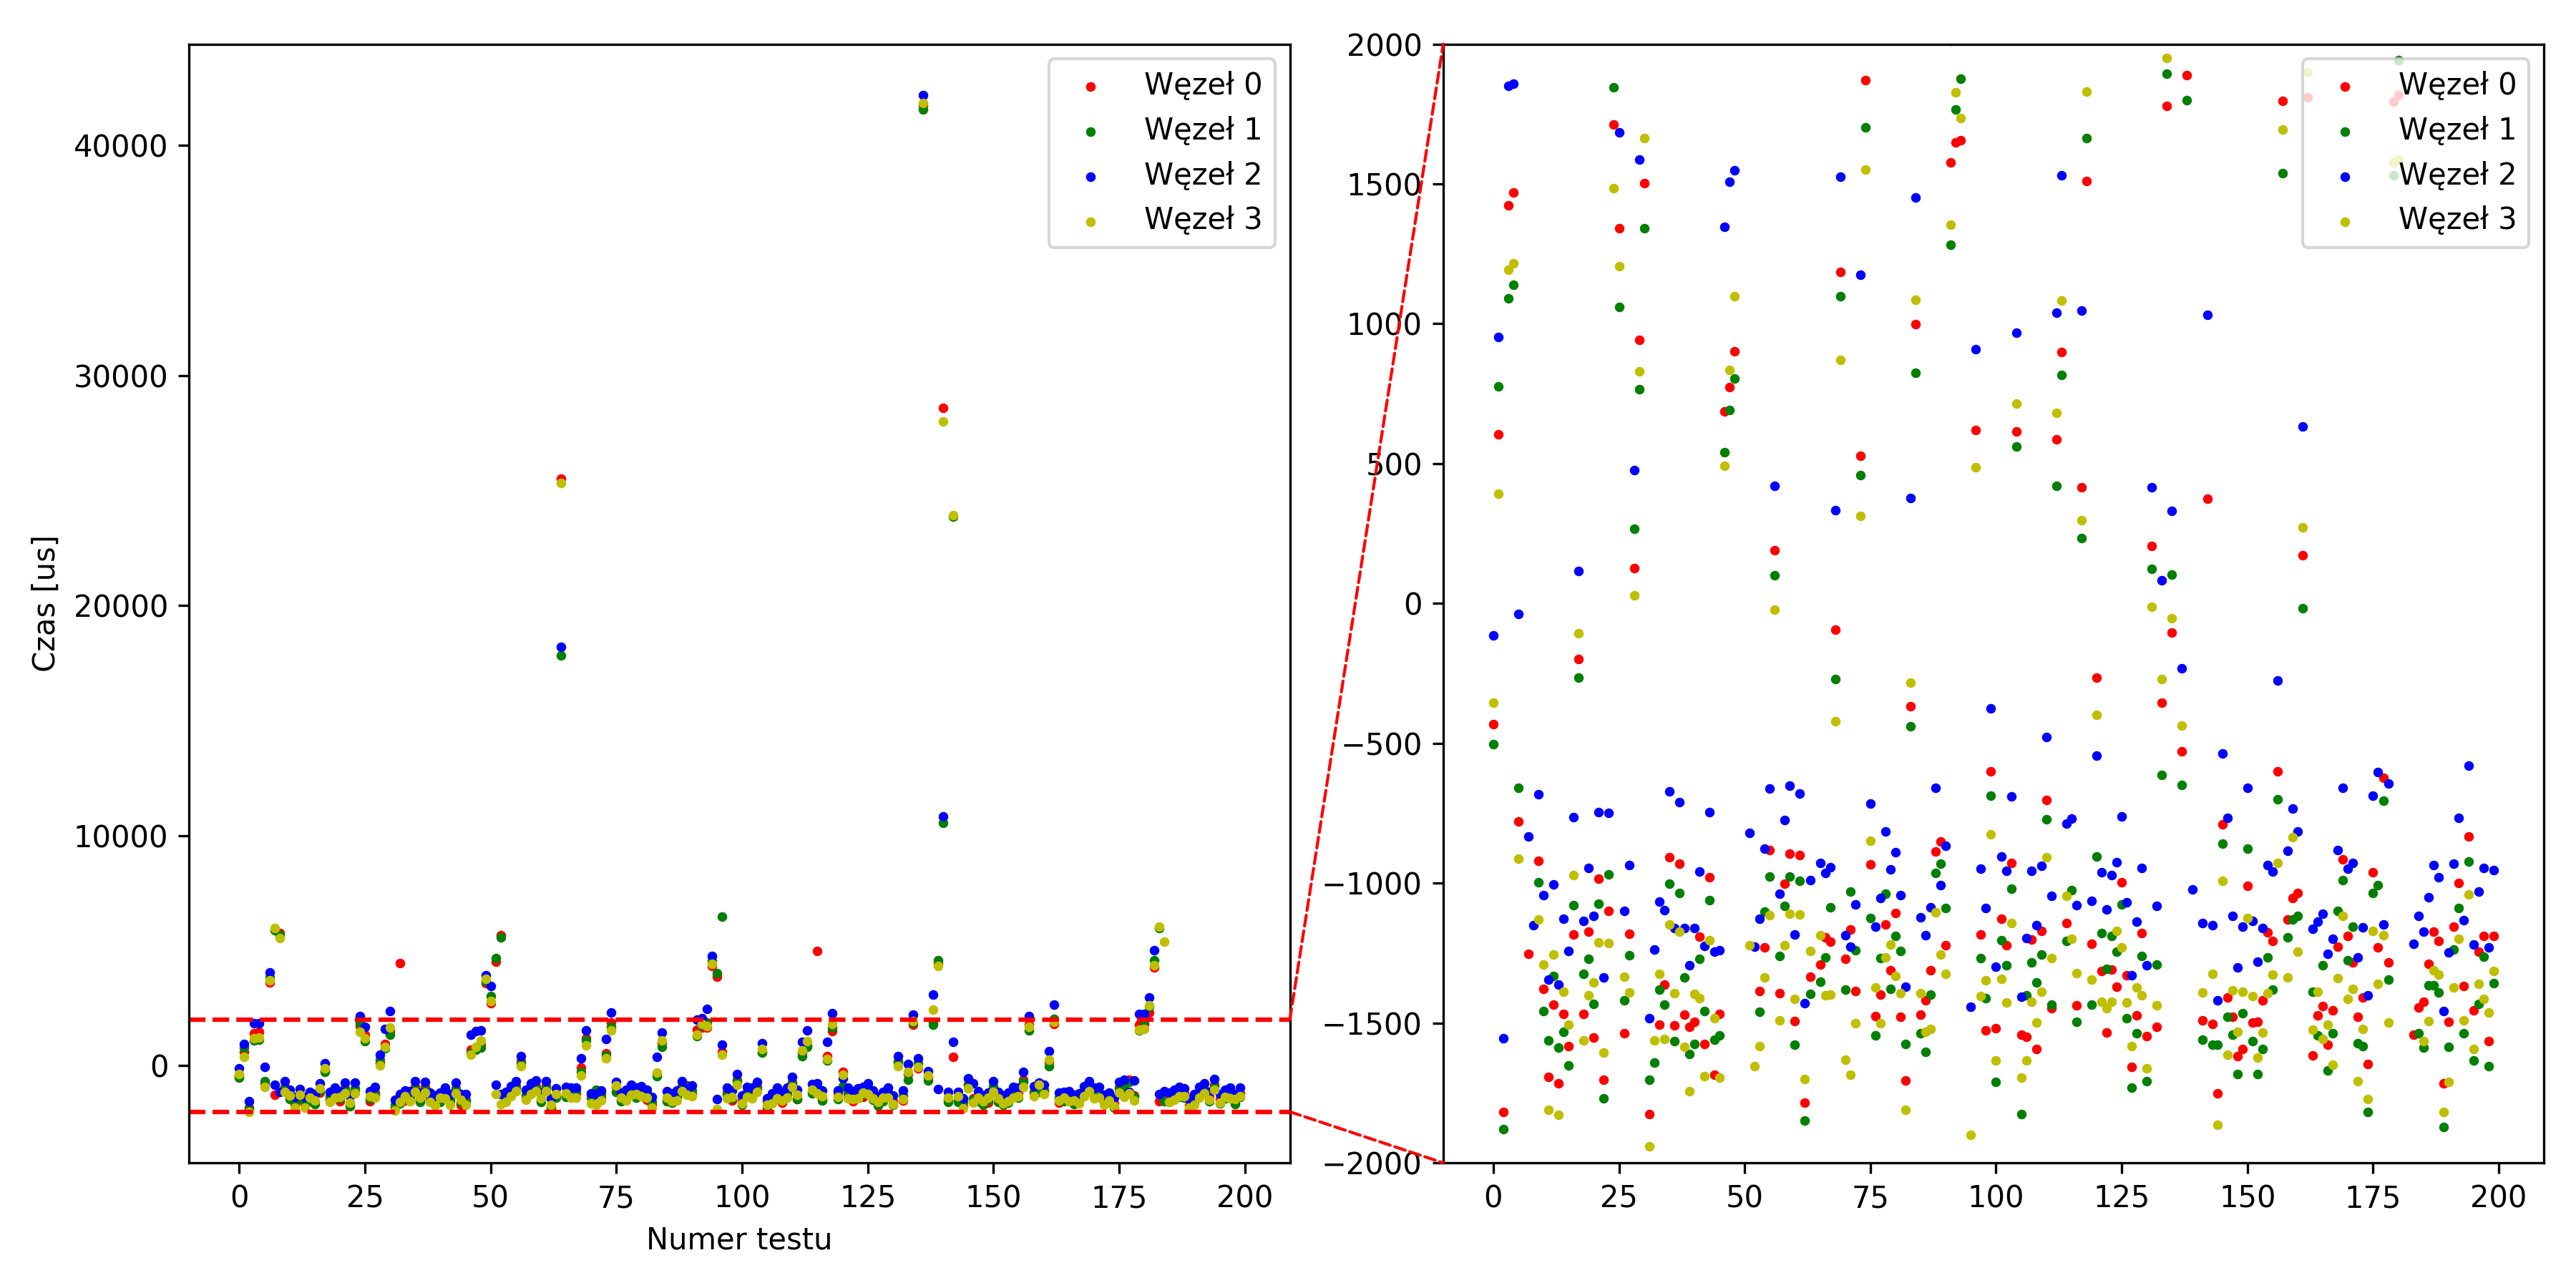
\includegraphics[width=.49\textwidth]{pics/time_deltas/time_deltas.png}
    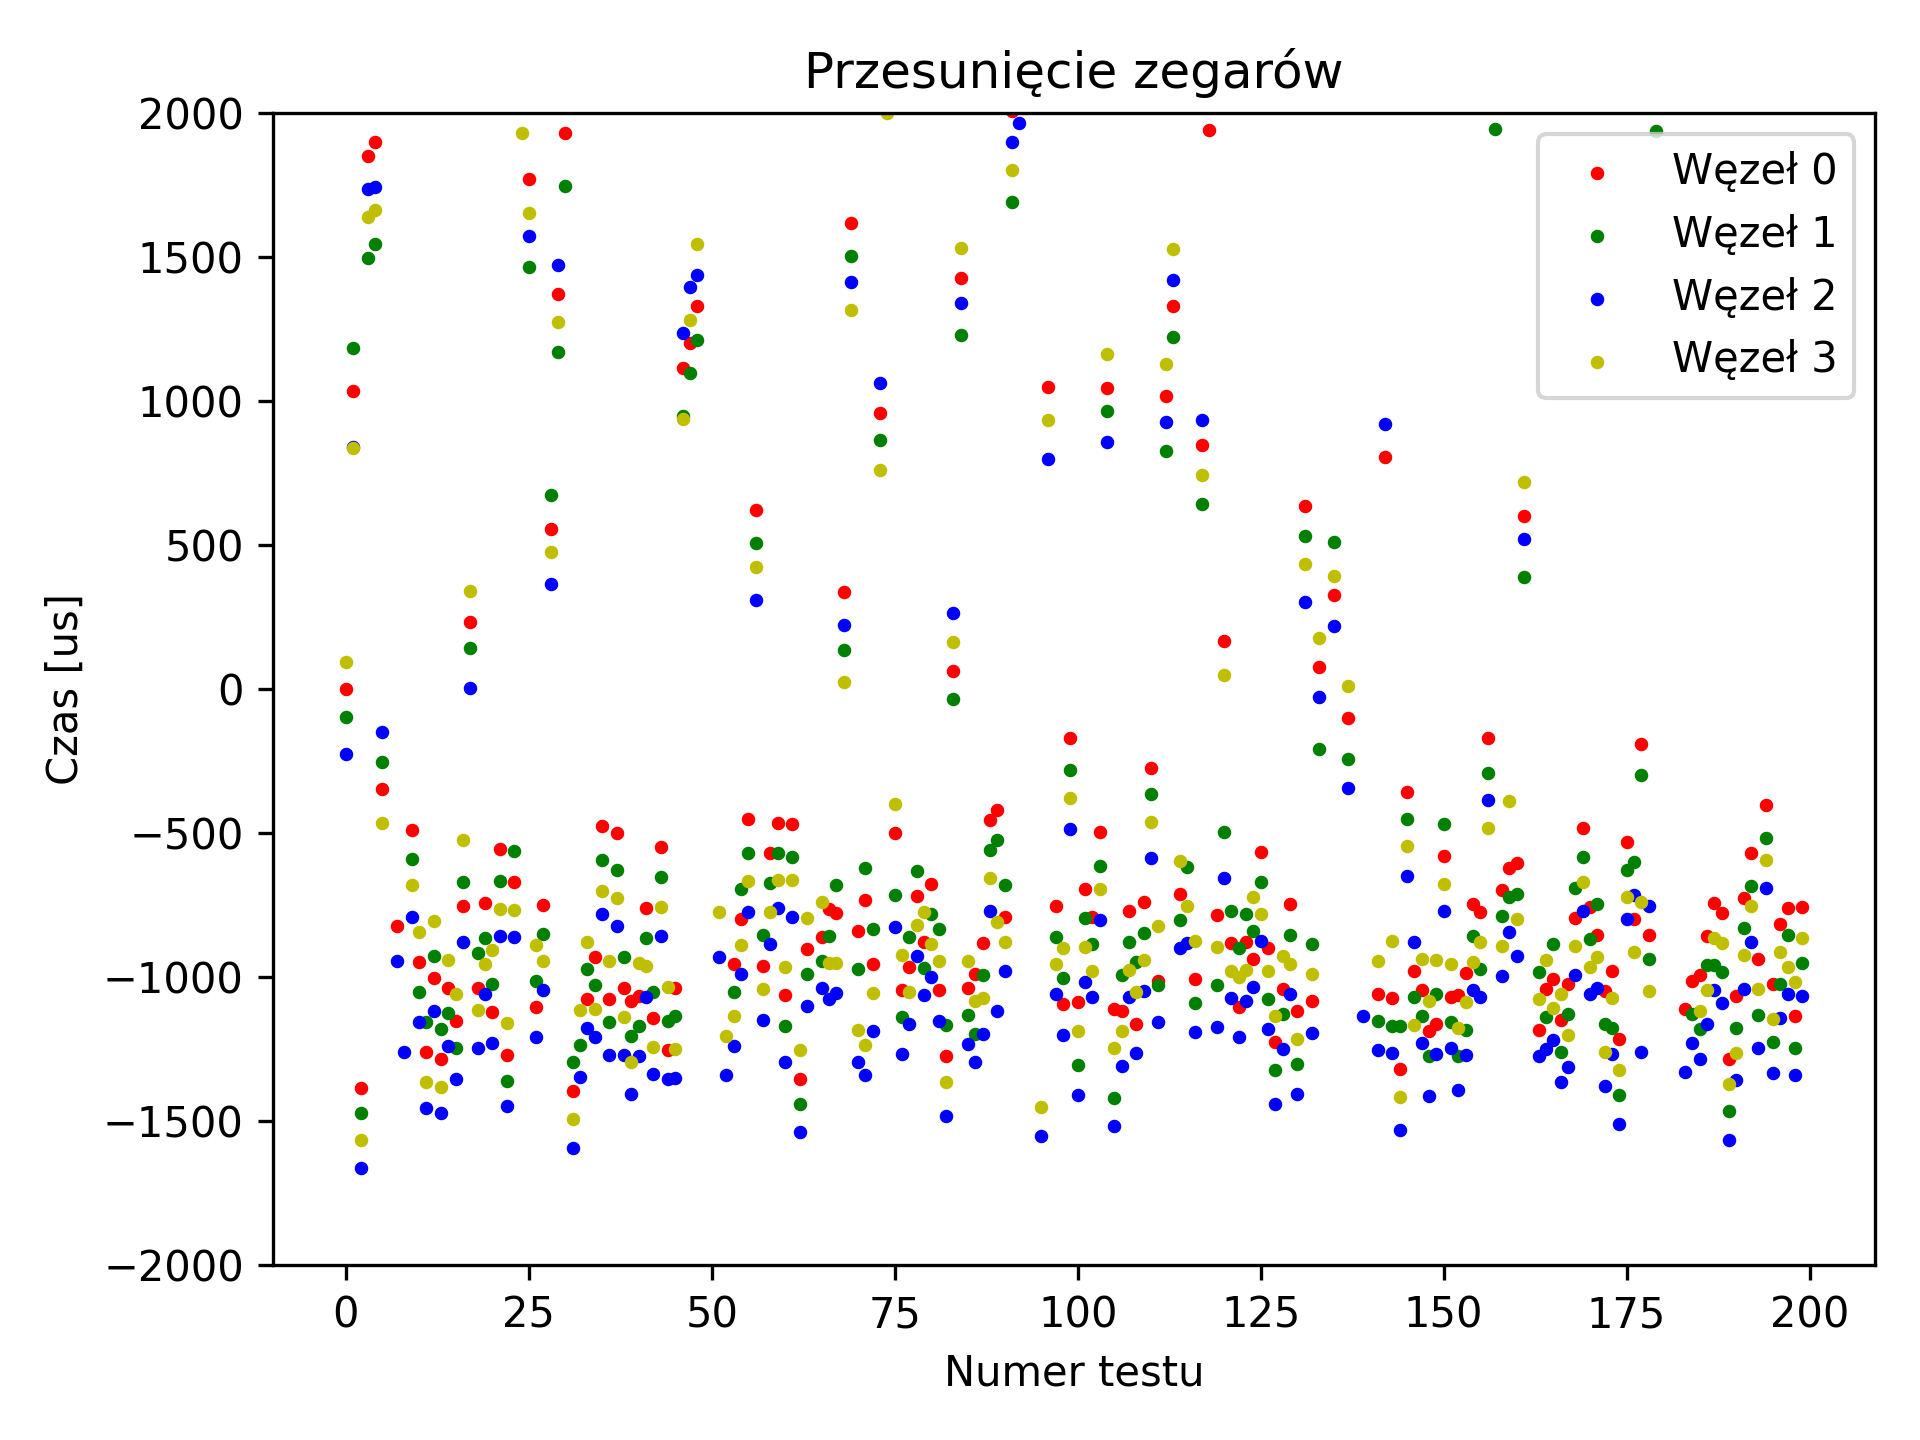
\includegraphics[width=.49\textwidth]{pics/time_deltas/time_deltas_close.png}
\caption{Wyniki pomiarów przesunięć zegarów}
\label{pic:offsets_deltas}
\end{figure}

\begin{figure}[h]
\centering
    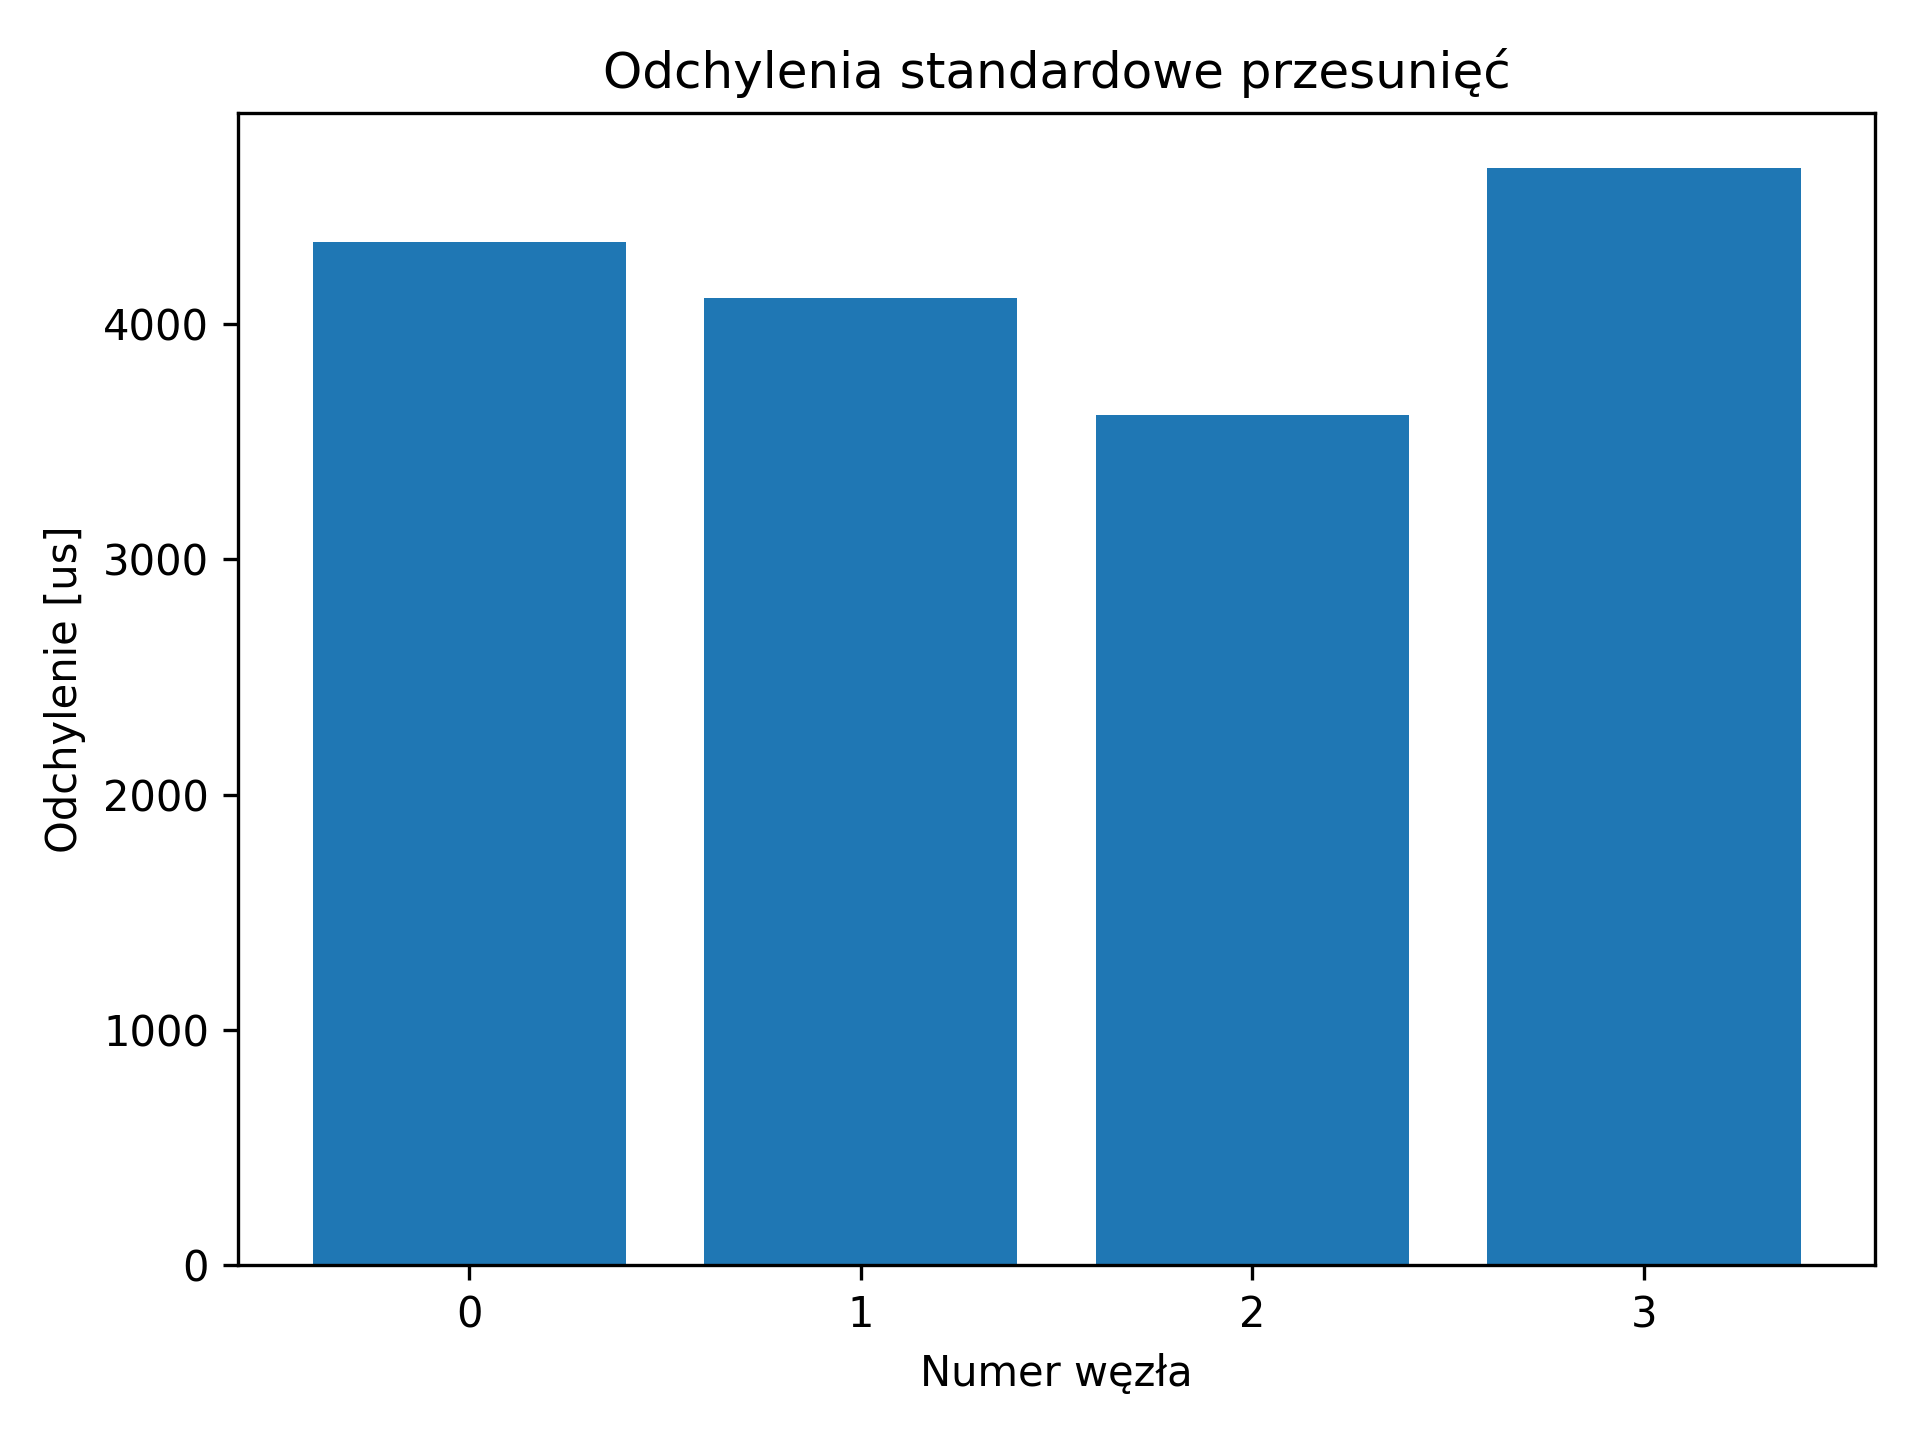
\includegraphics[width=.49\textwidth]{pics/time_deltas/stddev.png}
\caption{Odchylenia standardowe pomiarów}
\label{pic:stddev_deltas}
\end{figure}

Wykresy przesunięć wygenerowane na podstawie tych testów na pierwszy rzut oka są skoncentrowane podobnie jak poprzednie, jednakże odchylenie standardowe są prawie dwukrotnie mniejsze niż uprzednio, co daje nadzieje na bardziej wiarygodne wyniki. W porównaniu z pozostałymi sposobami brane będą pod uwagę wartości uśrednione.

\section{Synchronizacja sprzętowa}



\subsection{Synchronizacja z użyciem mikrofonów}

Innym pomysłem na synchronizację zegarów w węzłach było użycie mikrofonów, w które i tak węzły odbiorcze są wyposażone. Potrzebujmy znać jedynie przesunięcie względem zegara w węźle nadawczym dlatego wystarczającym będzie porównanie czasu nadania i odebrania sygnału dźwiękowego. Ponadto ten rodzaj synchronizacji w przeciwieństwie do synchronizacji programowej, która uzgadniała ze sobą jedynie zegary na podstawie wymienianych wiadomości, wlicza w czas transmisji wszelkie nie wzięte wcześniej pod uwagę opóźnienia, takie jak:

\begin{itemize}
    \item Czas pomiędzy wysłaniem wiadomości o nadaniu sygnału a zamknięciem kontaktora i poruszeniem membraną brzęczyka,
    \item Czas pomiędzy odebraniem sygnału przez mikrofon a zmianą stanu zmiennej na to wskazującej.
\end{itemize}


\begin{figure}[h]
\centering
    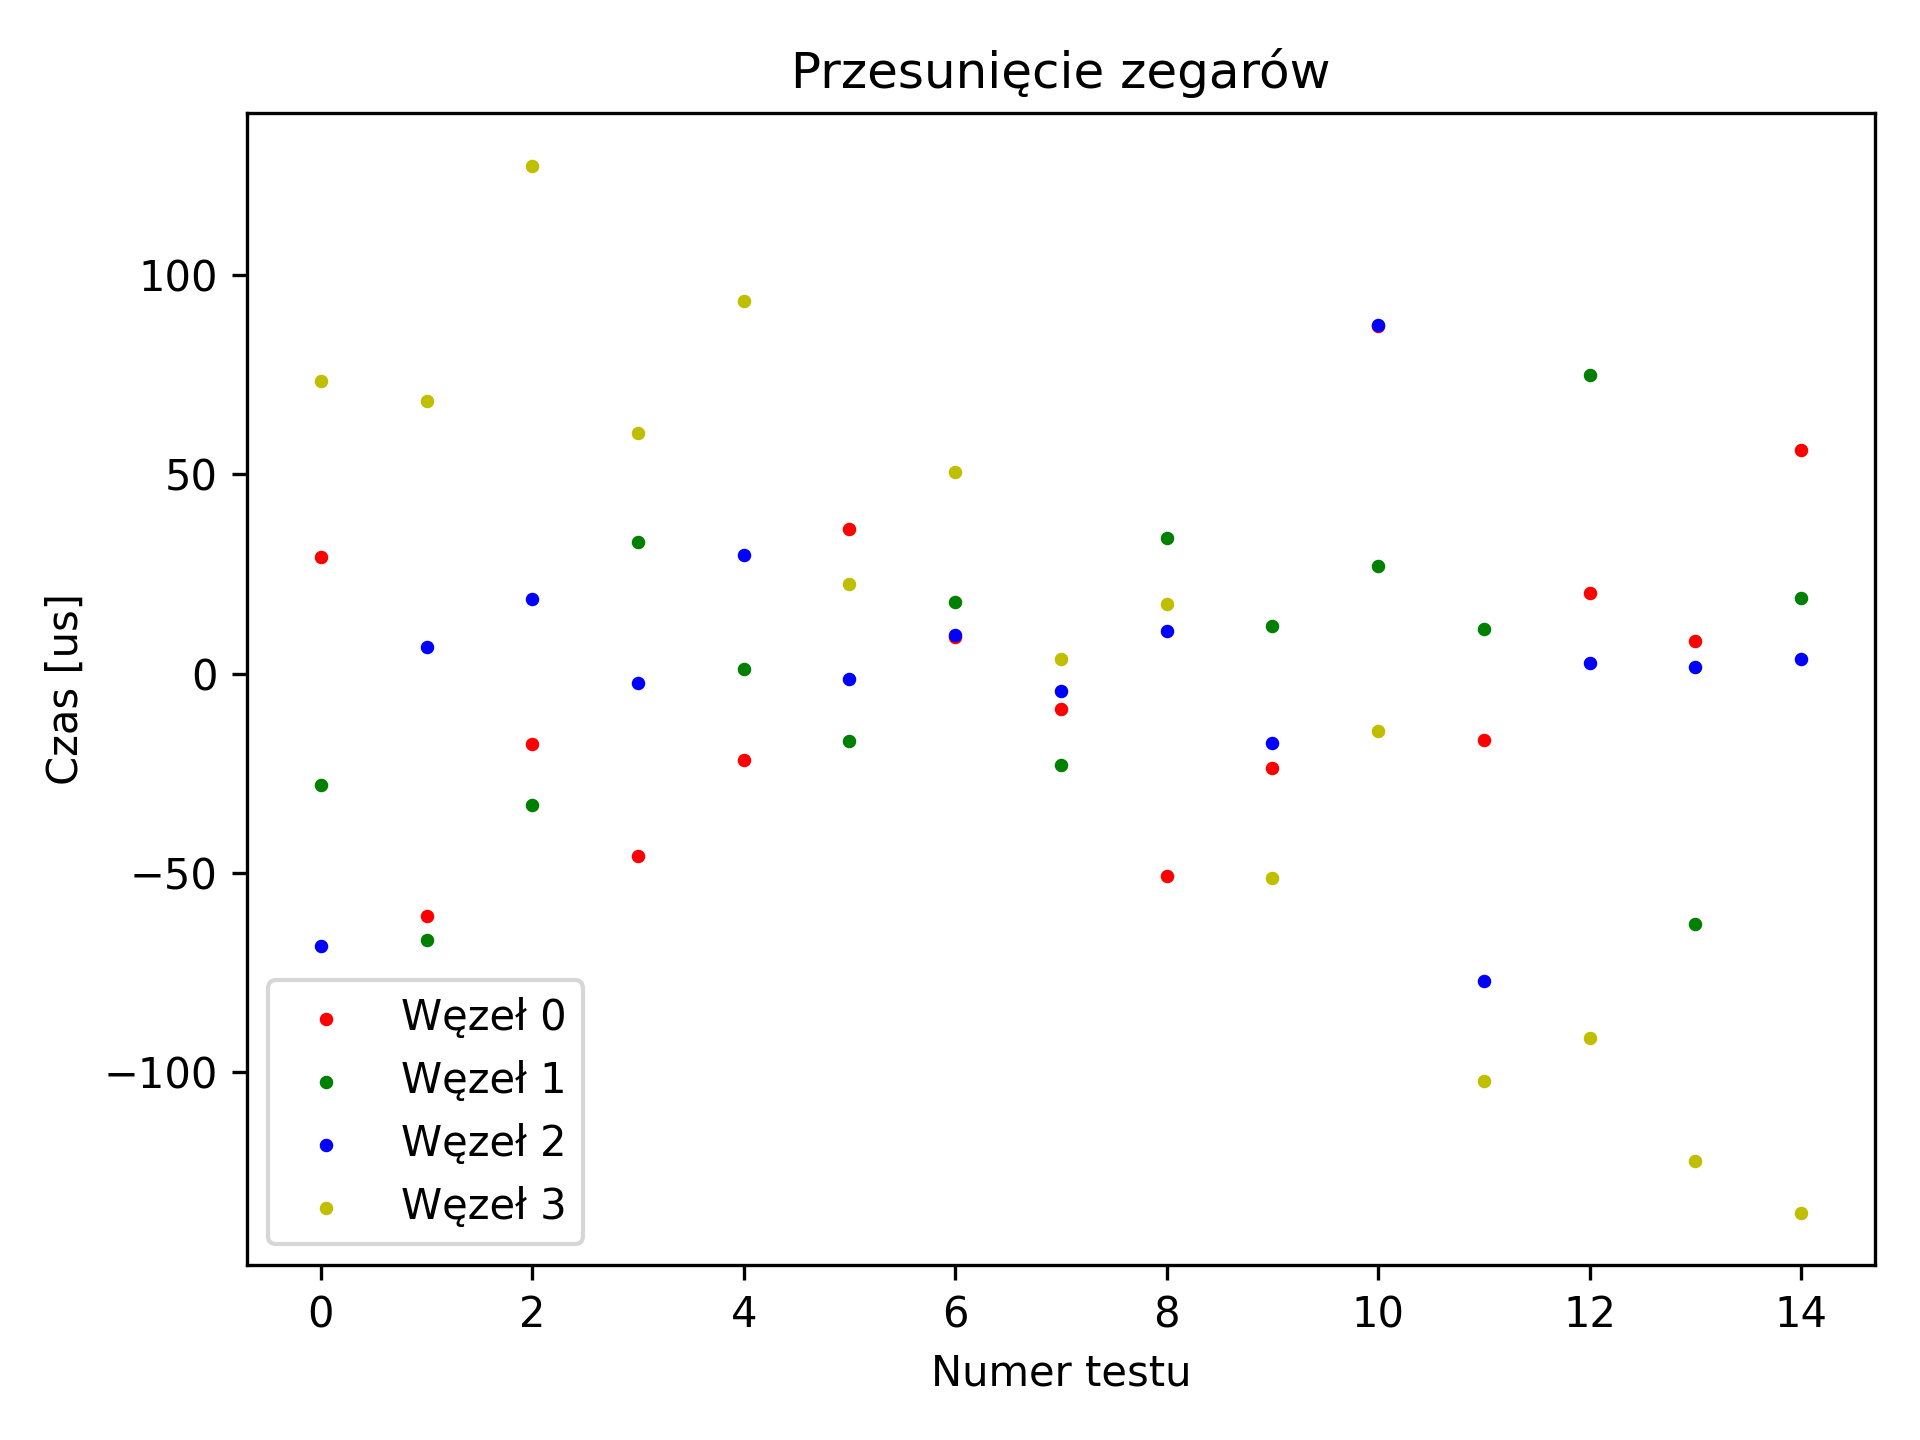
\includegraphics[width=.49\textwidth]{pics/mic_sync/offsets.png}
    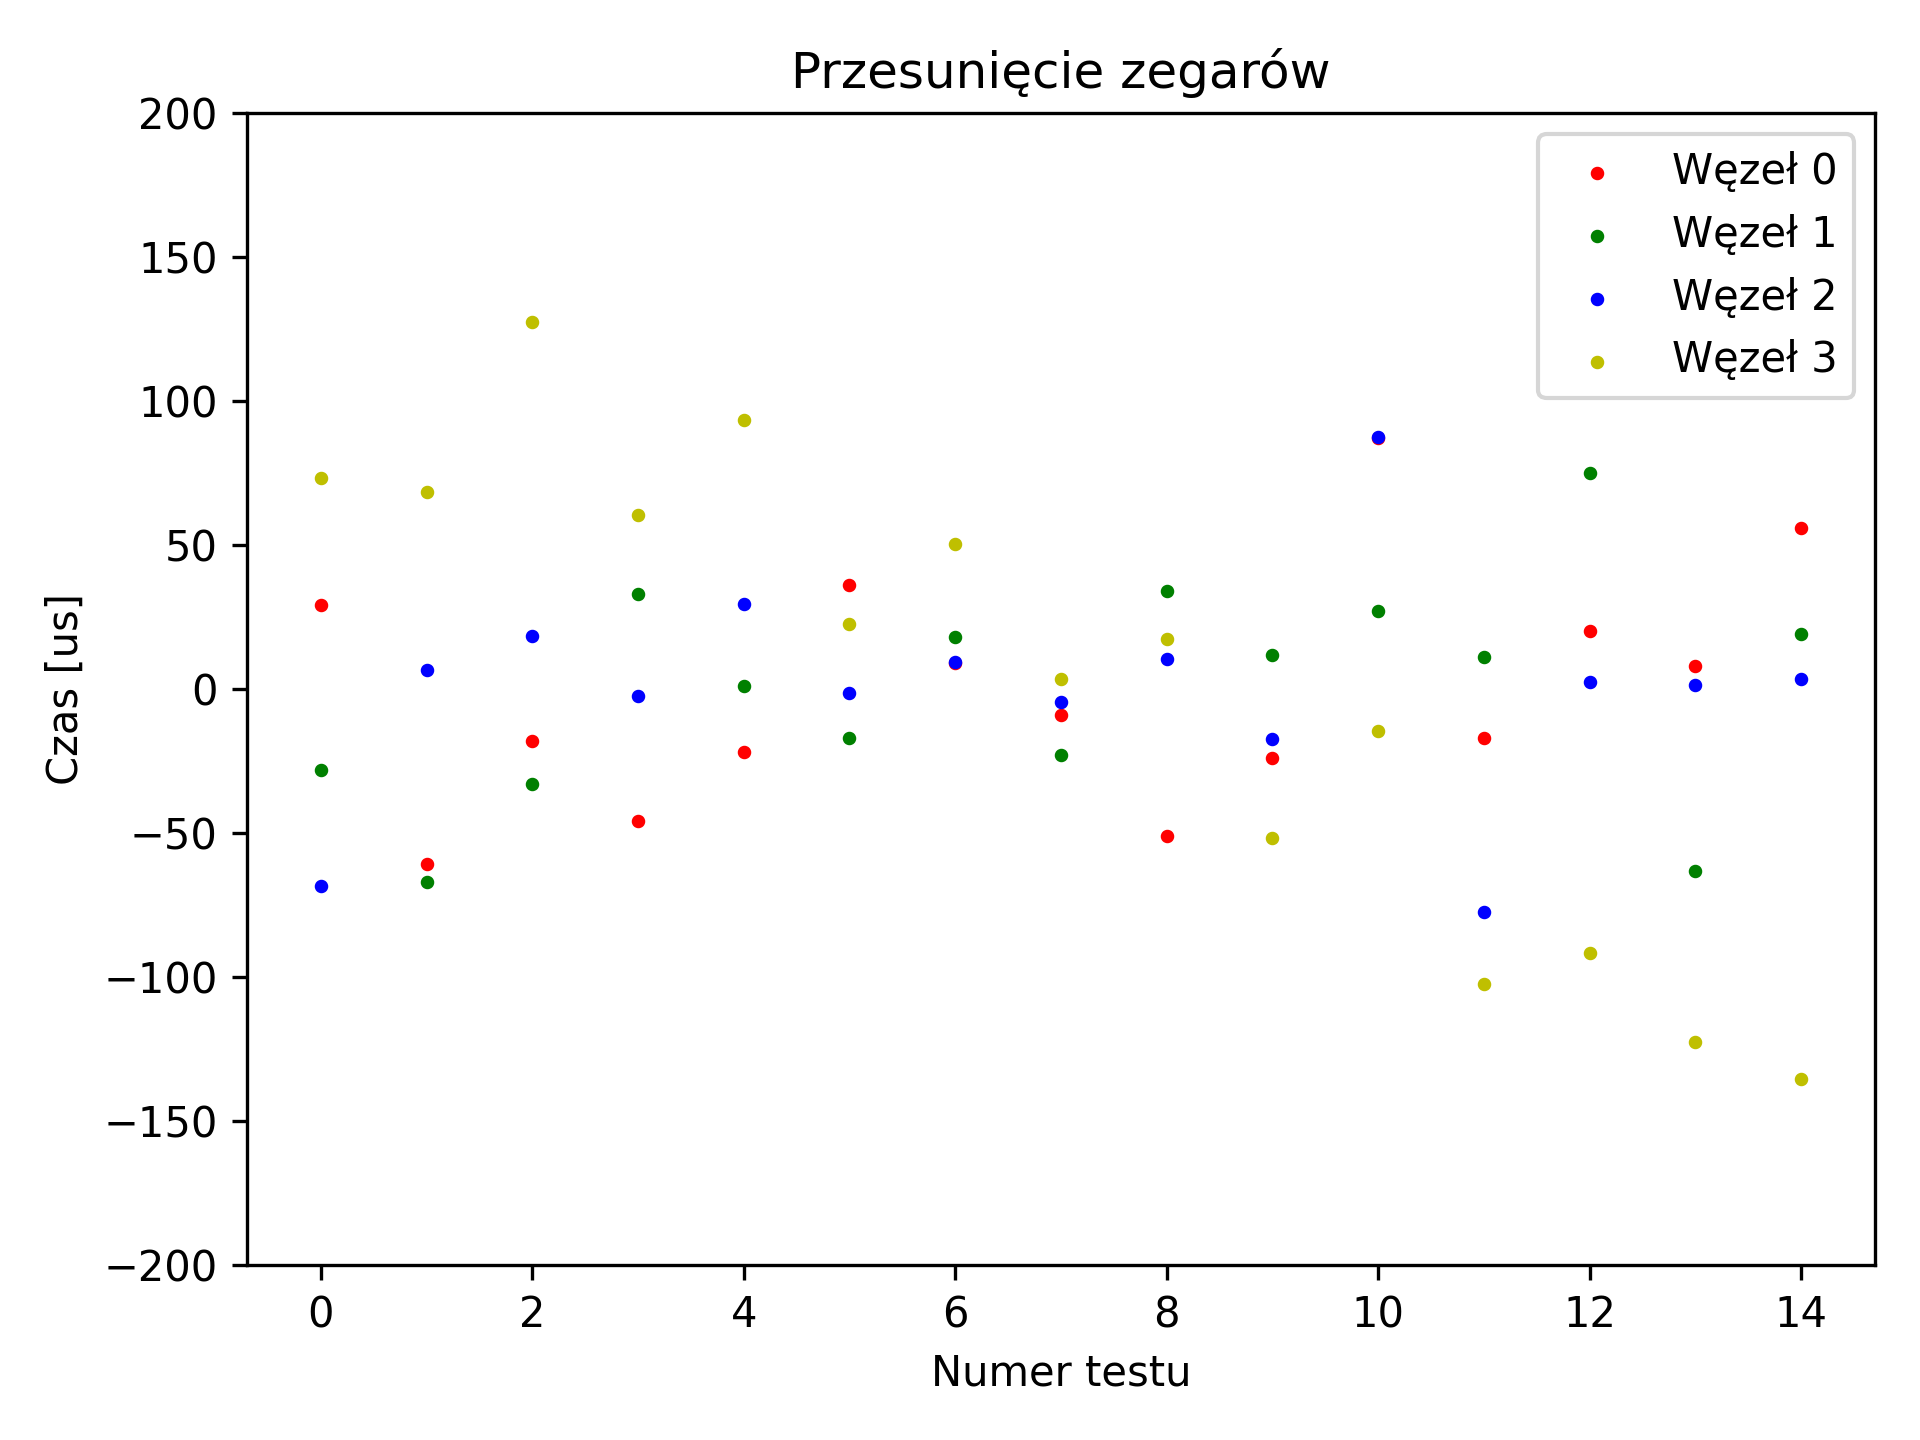
\includegraphics[width=.49\textwidth]{pics/mic_sync/offsets_close.png}
\caption{Wyniki pomiarów przesunięć zegarów}
\label{pic:offsets_mic}
\end{figure}

\begin{figure}[h]
\centering
    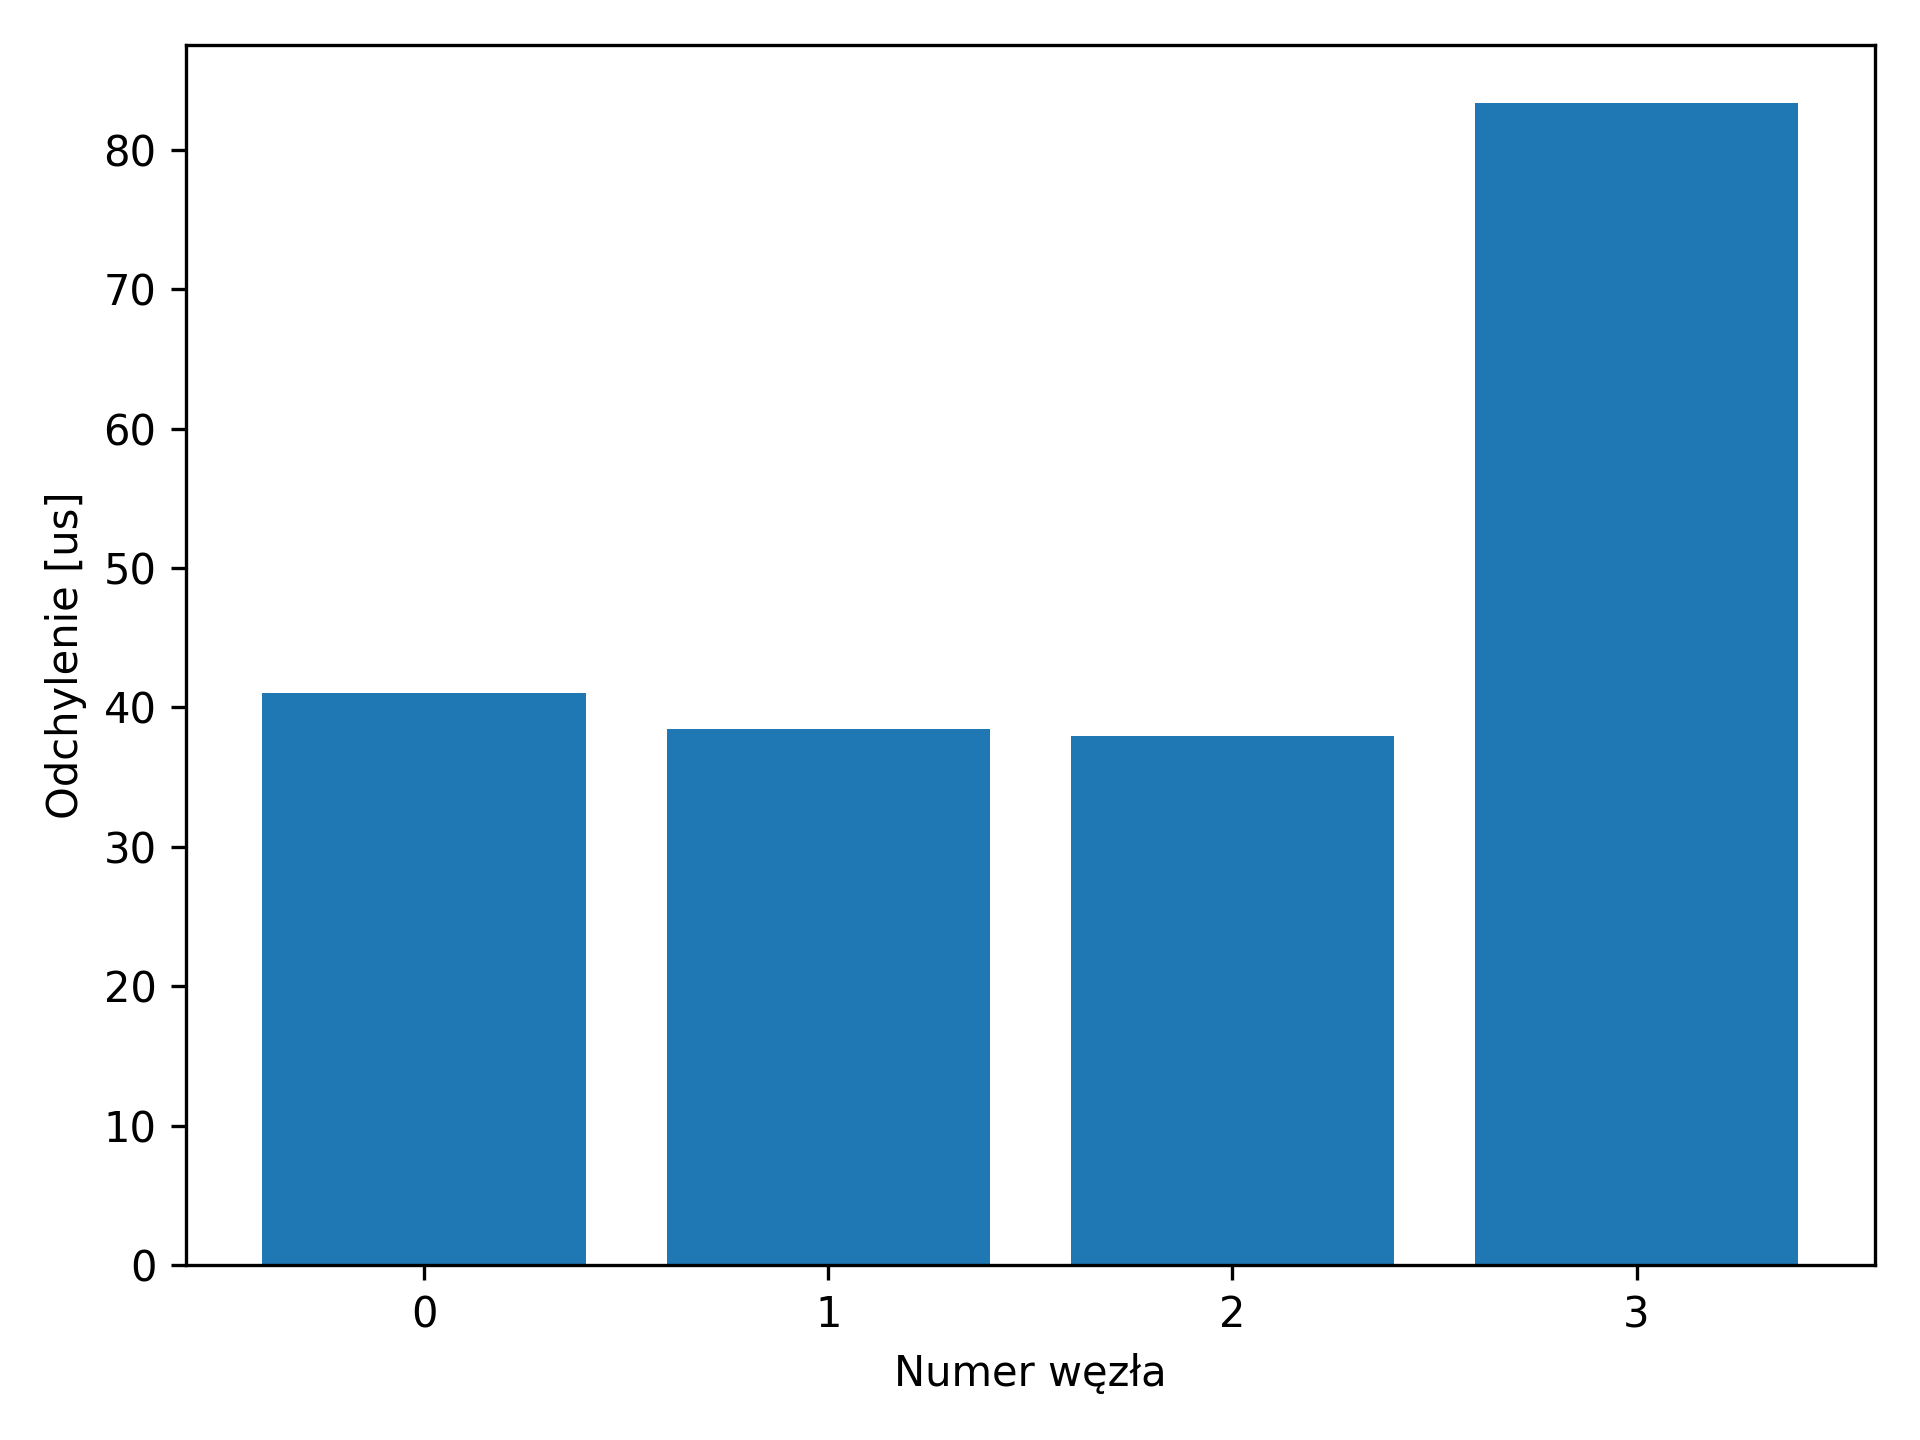
\includegraphics[width=.49\textwidth]{pics/mic_sync/stddev_offsets.png}
\caption{Odchylenia standardowe pomiarów}
\label{pic:stddev_mic}
\end{figure}